\PassOptionsToPackage{unicode=true}{hyperref} % options for packages loaded elsewhere
\PassOptionsToPackage{hyphens}{url}
\PassOptionsToPackage{dvipsnames,svgnames*,x11names*}{xcolor}
%
\documentclass[10pt,ignorenonframetext,]{beamer}
\usepackage{pgfpages}
\setbeamertemplate{caption}[numbered]
\setbeamertemplate{caption label separator}{: }
\setbeamercolor{caption name}{fg=normal text.fg}
\beamertemplatenavigationsymbolsempty
% Prevent slide breaks in the middle of a paragraph:
\widowpenalties 1 10000
\raggedbottom
\setbeamertemplate{part page}{
\centering
\begin{beamercolorbox}[sep=16pt,center]{part title}
  \usebeamerfont{part title}\insertpart\par
\end{beamercolorbox}
}
\setbeamertemplate{section page}{
\centering
\begin{beamercolorbox}[sep=12pt,center]{part title}
  \usebeamerfont{section title}\insertsection\par
\end{beamercolorbox}
}
\setbeamertemplate{subsection page}{
\centering
\begin{beamercolorbox}[sep=8pt,center]{part title}
  \usebeamerfont{subsection title}\insertsubsection\par
\end{beamercolorbox}
}
\AtBeginPart{
  \frame{\partpage}
}
\AtBeginSection{
  \ifbibliography
  \else
    \frame{\sectionpage}
  \fi
}
\AtBeginSubsection{
  \frame{\subsectionpage}
}
\usepackage{lmodern}
\usepackage{amssymb,amsmath}
\usepackage{ifxetex,ifluatex}
\usepackage{fixltx2e} % provides \textsubscript
\ifnum 0\ifxetex 1\fi\ifluatex 1\fi=0 % if pdftex
  \usepackage[T1]{fontenc}
  \usepackage[utf8]{inputenc}
  \usepackage{textcomp} % provides euro and other symbols
\else % if luatex or xelatex
  \usepackage{unicode-math}
  \defaultfontfeatures{Ligatures=TeX,Scale=MatchLowercase}
\fi
\usetheme[]{Singapore}
\usefonttheme{serif}
% use upquote if available, for straight quotes in verbatim environments
\IfFileExists{upquote.sty}{\usepackage{upquote}}{}
% use microtype if available
\IfFileExists{microtype.sty}{%
\usepackage[]{microtype}
\UseMicrotypeSet[protrusion]{basicmath} % disable protrusion for tt fonts
}{}
\IfFileExists{parskip.sty}{%
\usepackage{parskip}
}{% else
\setlength{\parindent}{0pt}
\setlength{\parskip}{6pt plus 2pt minus 1pt}
}
\usepackage{xcolor}
\usepackage{hyperref}
\hypersetup{
            pdftitle={Module 3: Linear Regression},
            pdfauthor={Stefanie Muff, Department of Mathematical Sciences, NTNU},
            colorlinks=true,
            linkcolor=Maroon,
            filecolor=Maroon,
            citecolor=Blue,
            urlcolor=blue,
            breaklinks=true}
\urlstyle{same}  % don't use monospace font for urls
\newif\ifbibliography
\usepackage{color}
\usepackage{fancyvrb}
\newcommand{\VerbBar}{|}
\newcommand{\VERB}{\Verb[commandchars=\\\{\}]}
\DefineVerbatimEnvironment{Highlighting}{Verbatim}{commandchars=\\\{\}}
% Add ',fontsize=\small' for more characters per line
\usepackage{framed}
\definecolor{shadecolor}{RGB}{248,248,248}
\newenvironment{Shaded}{\begin{snugshade}}{\end{snugshade}}
\newcommand{\AlertTok}[1]{\textcolor[rgb]{0.94,0.16,0.16}{#1}}
\newcommand{\AnnotationTok}[1]{\textcolor[rgb]{0.56,0.35,0.01}{\textbf{\textit{#1}}}}
\newcommand{\AttributeTok}[1]{\textcolor[rgb]{0.77,0.63,0.00}{#1}}
\newcommand{\BaseNTok}[1]{\textcolor[rgb]{0.00,0.00,0.81}{#1}}
\newcommand{\BuiltInTok}[1]{#1}
\newcommand{\CharTok}[1]{\textcolor[rgb]{0.31,0.60,0.02}{#1}}
\newcommand{\CommentTok}[1]{\textcolor[rgb]{0.56,0.35,0.01}{\textit{#1}}}
\newcommand{\CommentVarTok}[1]{\textcolor[rgb]{0.56,0.35,0.01}{\textbf{\textit{#1}}}}
\newcommand{\ConstantTok}[1]{\textcolor[rgb]{0.00,0.00,0.00}{#1}}
\newcommand{\ControlFlowTok}[1]{\textcolor[rgb]{0.13,0.29,0.53}{\textbf{#1}}}
\newcommand{\DataTypeTok}[1]{\textcolor[rgb]{0.13,0.29,0.53}{#1}}
\newcommand{\DecValTok}[1]{\textcolor[rgb]{0.00,0.00,0.81}{#1}}
\newcommand{\DocumentationTok}[1]{\textcolor[rgb]{0.56,0.35,0.01}{\textbf{\textit{#1}}}}
\newcommand{\ErrorTok}[1]{\textcolor[rgb]{0.64,0.00,0.00}{\textbf{#1}}}
\newcommand{\ExtensionTok}[1]{#1}
\newcommand{\FloatTok}[1]{\textcolor[rgb]{0.00,0.00,0.81}{#1}}
\newcommand{\FunctionTok}[1]{\textcolor[rgb]{0.00,0.00,0.00}{#1}}
\newcommand{\ImportTok}[1]{#1}
\newcommand{\InformationTok}[1]{\textcolor[rgb]{0.56,0.35,0.01}{\textbf{\textit{#1}}}}
\newcommand{\KeywordTok}[1]{\textcolor[rgb]{0.13,0.29,0.53}{\textbf{#1}}}
\newcommand{\NormalTok}[1]{#1}
\newcommand{\OperatorTok}[1]{\textcolor[rgb]{0.81,0.36,0.00}{\textbf{#1}}}
\newcommand{\OtherTok}[1]{\textcolor[rgb]{0.56,0.35,0.01}{#1}}
\newcommand{\PreprocessorTok}[1]{\textcolor[rgb]{0.56,0.35,0.01}{\textit{#1}}}
\newcommand{\RegionMarkerTok}[1]{#1}
\newcommand{\SpecialCharTok}[1]{\textcolor[rgb]{0.00,0.00,0.00}{#1}}
\newcommand{\SpecialStringTok}[1]{\textcolor[rgb]{0.31,0.60,0.02}{#1}}
\newcommand{\StringTok}[1]{\textcolor[rgb]{0.31,0.60,0.02}{#1}}
\newcommand{\VariableTok}[1]{\textcolor[rgb]{0.00,0.00,0.00}{#1}}
\newcommand{\VerbatimStringTok}[1]{\textcolor[rgb]{0.31,0.60,0.02}{#1}}
\newcommand{\WarningTok}[1]{\textcolor[rgb]{0.56,0.35,0.01}{\textbf{\textit{#1}}}}
\usepackage{graphicx,grffile}
\makeatletter
\def\maxwidth{\ifdim\Gin@nat@width>\linewidth\linewidth\else\Gin@nat@width\fi}
\def\maxheight{\ifdim\Gin@nat@height>\textheight\textheight\else\Gin@nat@height\fi}
\makeatother
% Scale images if necessary, so that they will not overflow the page
% margins by default, and it is still possible to overwrite the defaults
% using explicit options in \includegraphics[width, height, ...]{}
\setkeys{Gin}{width=\maxwidth,height=\maxheight,keepaspectratio}
\setlength{\emergencystretch}{3em}  % prevent overfull lines
\providecommand{\tightlist}{%
  \setlength{\itemsep}{0pt}\setlength{\parskip}{0pt}}
\setcounter{secnumdepth}{0}

% set default figure placement to htbp
\makeatletter
\def\fps@figure{htbp}
\makeatother


\title{Module 3: Linear Regression}
\providecommand{\subtitle}[1]{}
\subtitle{TMA4268 Statistical Learning V2021}
\author{Stefanie Muff, Department of Mathematical Sciences, NTNU}
\date{January 25 and 26, 2021}

\begin{document}
\frame{\titlepage}

\begin{frame}

Last update: January 25, 2021

\end{frame}

\begin{frame}{Acknowledgements}
\protect\hypertarget{acknowledgements}{}

\begin{itemize}
\item
  Thanks to Mette Langaas and her TAs who permit me to use and modify
  their original material.
\item
  Some of the figures and slides in this presentation are taken (or are
  inspired) from James et al. (2013).
\end{itemize}

\end{frame}

\begin{frame}{Introduction}
\protect\hypertarget{introduction}{}

\begin{block}{Learning material for this module}

\(~\)

\begin{itemize}
\tightlist
\item
  James et al. (2013): An Introduction to Statistical Learning, Chapter
  3 (skip 3.5).
\end{itemize}

\(~\)

We need more statistical theory than is presented in the textbook, which
you find in this module page.

\end{block}

\end{frame}

\begin{frame}

\begin{block}{What will you learn?}

\vspace{2mm}

\begin{itemize}
\tightlist
\item
  Simple linear regression:

  \begin{itemize}
  \tightlist
  \item
    Model and assumptions
  \item
    Least squares
  \item
    Testing and confidence intervals
  \end{itemize}
\end{itemize}

\vspace{2mm}

\begin{itemize}
\tightlist
\item
  Multiple linear regression:

  \begin{itemize}
  \tightlist
  \item
    The use of matrix algebra
  \item
    Distribution of estimators
  \item
    Assessing model fit, model selection
  \item
    Confidence and prediction ranges
  \end{itemize}
\end{itemize}

\vspace{2mm}

\begin{itemize}
\tightlist
\item
  Qualitative predictors
\end{itemize}

\vspace{2mm}

\begin{itemize}
\tightlist
\item
  Interactions
\end{itemize}

\vspace{2mm}

\begin{itemize}
\tightlist
\item
  Assessing model fit / residual analysis
\end{itemize}

\end{block}

\end{frame}

\begin{frame}{Linear regression}
\protect\hypertarget{linear-regression}{}

\begin{itemize}
\item
  Very simple approach for \emph{supervised learning}.
\item
  Parametric.
\item
  A quantitative response vs.~one or several explanatory variables
  (quantitative or qualitate).
\item
  Is linear regression too simple? Maybe, but very useful. Important to
  \emph{understand} because many learning methods can be seen as
  generalization of linear regression.
\end{itemize}

\end{frame}

\begin{frame}

\begin{block}{Motivating example: Prognostic factors for body fat}

\tiny(From Theo Gasser \& Burkhardt Seifert \emph{Grundbegriffe der
Biostatistik})

\vspace{2mm}
\normalsize

Body fat is an important indicator for overweight, but difficult to
measure.

\vspace{2mm}

\textbf{Question:} Which factors allow for precise estimation
(prediction) of body fat?

\vspace{2mm}

Study with 243 male participants, where body fat (\%) and BMI and other
predictors were measured. Some
scatterplots\footnote{The data to reproduce these plots and analyses can be found here: https://github.com/stefaniemuff/statlearning/tree/master/3LinReg/data}:

\begin{center}\includegraphics[width=1\linewidth]{3LinReg_files/figure-beamer/motivating-1} \end{center}

\end{block}

\end{frame}

\begin{frame}

For a good predictive model we need to dive into \emph{multiple linear
regression}. However, wer start with the simple case of \emph{only one
predictor variable}:

\begin{center}\includegraphics[width=0.7\linewidth]{3LinReg_files/figure-beamer/motivating2-1} \end{center}

\end{frame}

\begin{frame}[fragile]

\textbf{Interesting questions}

\begin{enumerate}
\tightlist
\item
  How good is BMI as a predictor for body fat?
\item
  How strong is this relationship?
\item
  Is the relationship linear?
\item
  Are also other variables associated with \texttt{bodyfat}?
\item
  How well can we predict the bodyfat of a person?
\end{enumerate}

\end{frame}

\begin{frame}{Simple Linear Regression}
\protect\hypertarget{simple-linear-regression}{}

\begin{itemize}
\item
  One quantitative response \(Y\) is modelled
\item
  from \emph{one covariate} \(x\) (=simple),
\item
  and the relationship between \(Y\) and \(x\) is assumed to be
  \emph{linear}.
\end{itemize}

\vspace{6mm}

If the relation between \(Y\) and \(x\) is perfectly linear, all
instances of \((x,Y)\), given by \((x_i,y_i)\), \(i= 1,\ldots, n\), lie
on a straight line and fulfill \[y_i = \beta_0 + \beta_1 x_i\ .\]

\end{frame}

\begin{frame}

But which is the ``true'' or ``best'' line, if the relationship is not
exact?

\begin{center}\includegraphics[width=0.6\linewidth]{3LinReg_files/figure-beamer/motivating3-1} \end{center}

\textbf{Task:} Estimate the intercept and slope parameters (by ``eye'')
and write it down (we will look at the ``best'' answer later).

Add your answer into the google sheet:
\url{https://docs.google.com/spreadsheets/d/1DishfNIsYmmcTmNjsTDGeyBK9FElC7yGpyYJoK32SyI/edit?usp=sharing}

\end{frame}

\begin{frame}

It is obvious that

\begin{itemize}
\tightlist
\item
  the linear relationship does not describe the data perfectly.
\item
  another realization of the data (other 243 males) would lead to a
  slightly different picture.
\end{itemize}

\vspace{4mm}

\(\Rightarrow\) We need a \textbf{model} that describes the relationship
between BMI and bodyfat.

\end{frame}

\begin{frame}

\begin{block}{The simple linear regression model}

\vspace{3mm}

In the linear regression model the dependent variable \(Y\) is related
to the independent variable \(x\) as

\[Y = \beta_0 + \beta_1 x + \varepsilon \ , \qquad \varepsilon \sim N(0,\sigma^2) \ .\]
\vspace{2mm}

In this formulation \(Y\) is a random variable
\(Y \sim N(\beta_0 + \beta_1 x, \sigma^2\)) where
\[Y \quad= \quad \underbrace{\text{ expected value }}_{\mathsf{E}(Y) = \beta_0 + \beta_1 x} \quad + \quad \underbrace{\text{ error}}_{\varepsilon}  \ .\]

Note:

\begin{itemize}
\tightlist
\item
  The model for \(Y\) given \(x\) has
  \emph{\textcolor{red}{three parameters}}: \(\beta_0\) (intercept),
  \(\beta_1\) (slope coefficient) and \(\sigma^2\) .
\item
  \(x\) is the \emph{\textcolor{red}{independent}}/
  \emph{\textcolor{red}{explanatory}} /
  \emph{\textcolor{red}{regressor}} variable.
\item
  \(Y\) is the \emph{\textcolor{red}{dependent}} /
  \emph{\textcolor{red}{outcome}} / \emph{\textcolor{red}{response}}
  variable.
\end{itemize}

\end{block}

\end{frame}

\begin{frame}

\begin{block}{Modeling assumptions}

\vspace{4mm}

The central assumption in linear regression is that for any pairs
(\(x_i,Y_i\)), the error \(\varepsilon_i \sim N(0,\sigma^2)\). This
implies \vspace{2mm}

\begin{enumerate}
[a)]
\item
  The expected value of \(\varepsilon_i\) is 0:
  \(\mathsf{E}(\varepsilon_i)=0\).
\item
  All \(\varepsilon_i\) have the same variance:
  \(\mathsf{Var}(\varepsilon_i)=\sigma^2\).
\item
  All \(\varepsilon_i\) are normally distributed.
\item
  \(\varepsilon\) is independent of any variable, observation number
  etc.
\item
  \(\varepsilon_1, \varepsilon_2, \ldots, \varepsilon_n\) are
  independent of each other.
\end{enumerate}

\end{block}

\end{frame}

\begin{frame}

\begin{block}{Visualization of the regression assumptions}

The assumptions about the linear regression model lie in the error term
\[\varepsilon \sim N(0,\sigma^2) \ . \]

\vspace{-2mm}

\includegraphics[width=11cm]{pictures/regrAssumptions.jpg}

Note: The true regression line goes through \(\mathsf{E}(Y)\).

\end{block}

\end{frame}

\begin{frame}

\begin{block}{Parameter estimation (``model fitting'')}

\vspace{2mm}

In a regression analysis, the task is to estimate the \textbf{regression
coefficients} \(\beta_0\), \(\beta_1\) and the \textbf{residual
variance} \(\sigma^2\) for a given set of \((x,y)\) data.

\vspace{4mm}

\begin{itemize}
\item
  \textbf{Problem:} For more than two points \((x_i,y_i)\),
  \(i=1,\ldots, n\), there is generally no perfectly fitting line.
  \vspace{2mm}
\item
  \textbf{Aim}: We want to find the parameters \((a,b)\) of the best
  fitting line \(Y = a + b x\).
\end{itemize}

\vspace{2mm}

\begin{itemize}
\tightlist
\item
  \textbf{Idea:} Minimize the deviations between the data points
  \((x_i,y_i)\) and the regression line.
\end{itemize}

\vspace{4mm}

But what are we actually going to minimize?

\end{block}

\end{frame}

\begin{frame}

\begin{block}{Least squares}

\vspace{2mm}

Remember the \textbf{Least Squared Method}. Graphically, we are
minimizing the sum of the squared distances over all points:

\vspace{4mm}

\begin{center}\includegraphics[width=0.8\linewidth]{3LinReg_files/figure-beamer/squares-1} \end{center}

\end{block}

\end{frame}

\begin{frame}

\begin{itemize}
\tightlist
\item
  Mathematically, \(a\) and \(b\) are estimated such that the sum of
  \emph{\textcolor{red}{squared vertical distances}} (residual sum of
  squares)
\end{itemize}

\[\text{RSS} = \sum_{i=1}^n e_i^2 \ , \qquad \text{where} \quad e_i = y_i - (a + b x_i) \]

is being minimized.

\begin{itemize}
\item
  The respective ``best'' estimates are called \(\hat{\beta_0}\) and
  \(\hat{\beta_1}\).
\item
  We can predict the value of the response for a (new) observation of
  the covariate at \(x\). \[\hat{y} = \hat{\beta}_0 + \hat{\beta_1}x.\]
\item
  The \(i\)-th \emph{residual} of the model is the difference between
  the \(i\)-th \emph{observed} response value and the \(i\)-th
  \emph{predicted} value, and is written as: \[e_i = Y_i - \hat{y}_i.\]
\item
  We may regard the residuals as \emph{predictions} (not estimates) of
  the error terms \(\varepsilon_i\).
\end{itemize}

\tiny

(The error terms are random variables and can not be estimated - they
can be predicted. It is only for parameters that we speak about
estimates.)

\end{frame}

\begin{frame}

\begin{block}{Least squares estimators:}

\vspace{2mm}

Using \(n\) observed independent data points
\[(x_1,y_1), (x_2,y_2), \ldots, (x_n,y_n)\ ,\]

the least squares estiamtes for simple linear regression are given as

\begin{equation}\label{eq:beta0}
\hat{\beta}_0 = \bar{y}-\hat{\beta}_1 \bar{x}
\end{equation} and \begin{equation}\label{eq:beta1}
\hat{\beta}_1 = \frac{\sum_{i=1}^n(x_i-\bar{x})(y_i-\bar{y})}{\sum_{i=1}^n(x_i-\bar{x})^2} = \frac{\mathsf{Cov}(\boldsymbol{x},\boldsymbol{y})}{\mathsf{Var}(\boldsymbol{x})}\ ,
\end{equation}

\vspace{2mm}

where \(\bar{y} = \frac{1}{n} \sum_{i=1}^n y_i\) and
\(\bar{x} = \frac{1}{n}\sum_{i=1}^n x_i\) are the sample means.

\vspace{6mm}
\scriptsize

This is something you should have proven in your previous statistics
classes; if you forgot how to get there, please check again, e.g.~in
chapter 11 of the book by Walepole et al. (2012), see
\href{https://github.com/stefaniemuff/statlearning/blob/master/literature/Walepole_book.pdf}{here}.

\end{block}

\end{frame}

\begin{frame}

\begin{block}{Do-it-yourself ``by hand''}

\vspace{6mm}

Go to the Shiny gallery and try to ``estimate'' the correct parameters.
\vspace{2mm}

You can do this here: \vspace{2mm}

\url{https://gallery.shinyapps.io/simple_regression/}

\end{block}

\end{frame}

\begin{frame}[fragile]

\begin{block}{Example continued: Body fat}

\vspace{2mm}

Assume a linear relationship between the \% bodyfat (\texttt{bodyfat})
and the BMI (\texttt{bmi}), we can get the LS estimates using R as
follows:

\(~\)

\scriptsize

\begin{Shaded}
\begin{Highlighting}[]
\NormalTok{r.bodyfat =}\StringTok{ }\KeywordTok{lm}\NormalTok{(bodyfat }\OperatorTok{~}\StringTok{ }\NormalTok{bmi, }\DataTypeTok{data =}\NormalTok{ d.bodyfat)}
\end{Highlighting}
\end{Shaded}

\(~\)

\normalsize

The estimates (and more information) can be obtained as follows:

\(~\)

\scriptsize

\begin{Shaded}
\begin{Highlighting}[]
\KeywordTok{summary}\NormalTok{(r.bodyfat)}\OperatorTok{$}\NormalTok{coef}
\end{Highlighting}
\end{Shaded}

\begin{verbatim}
##               Estimate Std. Error   t value     Pr(>|t|)
## (Intercept) -26.984368  2.7689004 -9.745518 3.921511e-19
## bmi           1.818778  0.1083411 16.787522 2.063854e-42
\end{verbatim}

\end{block}

\end{frame}

\begin{frame}[fragile]

We see that the model fits the data quite well. It captures the essence.
It looks that a linear relationship between \texttt{bodyfat} and
\texttt{bmi} is a good approximation.

\begin{center}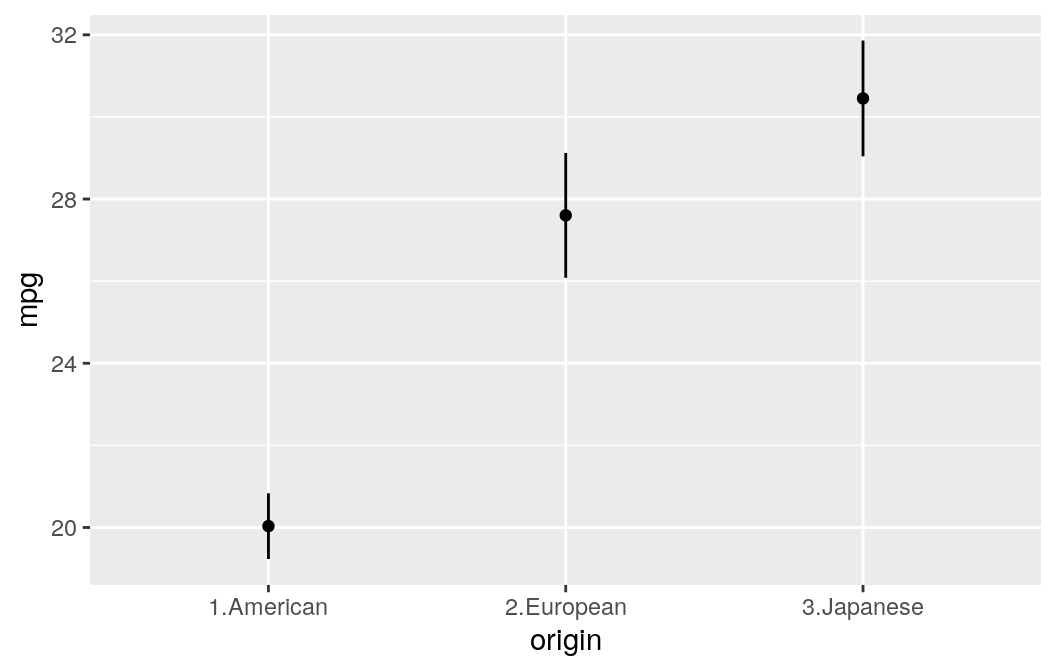
\includegraphics[width=0.8\linewidth]{3LinReg_files/figure-beamer/unnamed-chunk-3-1} \end{center}

\end{frame}

\begin{frame}

\textbf{Questions:}

\begin{itemize}
\item
  The blue line gives the estimated model. Explain what the line means
  in practice. Is this result plausible?
\item
  Compare the estimates for \(\beta_0\) and \(\beta_1\) to the estimates
  you gave at the beginning - were you close?
\item
  How does this relate to the \emph{true} (population) model?
\item
  \textbf{What could the regression line look like if another set of 243
  males were used for estimation?}
\end{itemize}

\end{frame}

\begin{frame}[fragile]

\begin{block}{Uncertainty in the estimates \(\hat\beta_0\) and
\(\hat\beta_1\)}

\vspace{2mm}

Note: \(\hat\beta_0\) and \(\hat\beta_1\) are themselves
\emph{\textcolor{red}{random variables}} and as such contain
\emph{\textcolor{red}{uncertainty}}!

\vspace{4mm}

Let us look again at the regression output, this time only for the
coefficients. The second column shows the standard error of the
estimate: \vspace{2mm}

\scriptsize

\begin{Shaded}
\begin{Highlighting}[]
\KeywordTok{summary}\NormalTok{(r.bodyfat)}\OperatorTok{$}\NormalTok{coef}
\end{Highlighting}
\end{Shaded}

\begin{verbatim}
##               Estimate Std. Error   t value     Pr(>|t|)
## (Intercept) -26.984368  2.7689004 -9.745518 3.921511e-19
## bmi           1.818778  0.1083411 16.787522 2.063854e-42
\end{verbatim}

\normalsize

\(~\)

\(\rightarrow\) The logical next question is: what is the distribution
of the estimates?

\end{block}

\end{frame}

\begin{frame}[fragile]

\begin{block}{Distribution of the estimators for \(\hat\beta_0\) and
\(\hat\beta_1\)}

\vspace{2mm}

To obtain an intuition, we generate data points according to model

\[y_i = 4 - 2x_i + \varepsilon_i \ , \quad \varepsilon_i\sim N(0,0.5^2). \]
In each round, we estimate the parameters and store them: \tiny

\begin{Shaded}
\begin{Highlighting}[]
\KeywordTok{set.seed}\NormalTok{(}\DecValTok{1}\NormalTok{)}
\NormalTok{niter <-}\StringTok{ }\DecValTok{1000}
\NormalTok{pars <-}\StringTok{ }\KeywordTok{matrix}\NormalTok{(}\OtherTok{NA}\NormalTok{, }\DataTypeTok{nrow =}\NormalTok{ niter, }\DataTypeTok{ncol =} \DecValTok{2}\NormalTok{)}
\ControlFlowTok{for}\NormalTok{ (ii }\ControlFlowTok{in} \DecValTok{1}\OperatorTok{:}\NormalTok{niter) \{}
\NormalTok{    x <-}\StringTok{ }\KeywordTok{rnorm}\NormalTok{(}\DecValTok{100}\NormalTok{)}
\NormalTok{    y <-}\StringTok{ }\DecValTok{4} \OperatorTok{-}\StringTok{ }\DecValTok{2} \OperatorTok{*}\StringTok{ }\NormalTok{x }\OperatorTok{+}\StringTok{ }\KeywordTok{rnorm}\NormalTok{(}\DecValTok{100}\NormalTok{, }\DecValTok{0}\NormalTok{, }\DataTypeTok{sd =} \FloatTok{0.5}\NormalTok{)}
\NormalTok{    pars[ii, ] <-}\StringTok{ }\KeywordTok{lm}\NormalTok{(y }\OperatorTok{~}\StringTok{ }\NormalTok{x)}\OperatorTok{$}\NormalTok{coef}
\NormalTok{\}}
\end{Highlighting}
\end{Shaded}

\normalsize Doing it 1000 times, we obtain the following distributions
for \(\hat\beta_0\) and \(\hat\beta_1\):

\begin{center}\includegraphics[width=0.4\linewidth]{3LinReg_files/figure-beamer/sim_fig-1} \end{center}

\end{block}

\end{frame}

\begin{frame}

\begin{block}{Accuracy of the parameter estimates}

\vspace{2mm}

\begin{itemize}
\item
  The standard errors of the estimates are given by the following
  formulas:
  \[\mathsf{Var}(\hat{\beta}_0)=\text{SE}(\hat{\beta}_0)^2 = \sigma^2 \Big [ \frac{1}{n} + \frac{\bar{x}^2}{\sum_{i=1}^n (x_i -\bar{x})^2} \Big]\]
  and
  \[\mathsf{Var}(\hat{\beta}_1)=\text{SE}(\hat{\beta}_1)^2 = \frac{\sigma^2}{\sum_{i=1}^n (x_i-\bar{x})^2}.\]
\item
  \(\mathsf{Cov}(\hat{\beta_0},\hat{\beta_1})\) is in general different
  from zero.
\end{itemize}

\(~\) \(~\)

\textbf{Note}: We will \emph{derive a general version} of these formulas
for multiple linear regression, because without matrix notation this is
very cumbersome.

\end{block}

\end{frame}

\begin{frame}

Under the assumption that \(\varepsilon \sim N(0,\sigma^2)\), and
assuming \(\hat\beta_0\) and \(\hat\beta_1\) are estimated as in
formulas (1) and (2), we have in addition that

\[
 \hat\beta_0 \sim N(\beta_0,{\sigma^{2}_{\beta_0}}) \quad \text{and} \quad \hat\beta_1 \sim N(\beta_1,{\sigma^{2}_{\beta_1}}) \ .
\]

\vspace{6mm}

\textbf{Again}: We will derive this in the multiple linear regression
version in more generality.

\end{frame}

\begin{frame}

\begin{block}{Design issue with data collection}

\vspace{2mm}

Recall that

\[\text{SE}(\hat{\beta}_1)^2 = \frac{\sigma^2}{\sum_{i=1}^n (x_i-\bar{x})^2} \ ,\]

thus for a given \(\sigma^2\), the standard error is only dependent on
the \emph{design} of the \(x_i\)'s!

\vspace{2mm}

\begin{itemize}
\item
  Would we like the \(\text{SE}(\hat{\beta}_1)^2\) large or small? Why?
\item
  If it is possible for us to choose the \(x_i\)'s, which strategy
  should we use to choose them?
\end{itemize}

\vspace{4cm}

\end{block}

\end{frame}

\begin{frame}

\begin{block}{Residual standard error (RSE)}

\vspace{2mm}

\begin{itemize}
\item
  \textbf{Problem}: \(\sigma\) is usually not known, but needs to be
  estimated\footnote{$\sigma^2$ is the \emph{irreducible error} variance.}.
\item
  Remember: The residual sum of squares is
  \(\text{RSS}=\sum_{i=1}^n (y_i-\hat{\beta}_0-\hat{\beta_1}x_{i})^2\).
\item
  An estimate of \(\sigma\), the residual standard error, RSE, is given
  by
  \[\hat\sigma = \text{RSE}  =\sqrt{\frac{1}{n-2} \text{RSS}} = \sqrt{\frac{1}{n-2}\sum_{i=1}^n (y_i -\hat{y}_i)^2} \ .\]
\item
  So actually we have
\end{itemize}

\[\hat{\text{SE}}(\hat{\beta}_1)^2 = \frac{{\hat\sigma}^2}{\sum_{i=1}^n (x_i-\bar{x})^2} \ ,\]
but we usually just write \({\text{SE}}(\hat{\beta}_1)^2\) (without the
extra hat).

\end{block}

\end{frame}

\begin{frame}[fragile]

The estimated standard errors can be seen using the \texttt{summary()}
function:

\(~\)

\scriptsize

\begin{Shaded}
\begin{Highlighting}[]
\KeywordTok{summary}\NormalTok{(r.bodyfat)}\OperatorTok{$}\NormalTok{coef}
\end{Highlighting}
\end{Shaded}

\begin{verbatim}
##               Estimate Std. Error   t value     Pr(>|t|)
## (Intercept) -26.984368  2.7689004 -9.745518 3.921511e-19
## bmi           1.818778  0.1083411 16.787522 2.063854e-42
\end{verbatim}

\end{frame}

\begin{frame}{Testing and Confidence Intervals}
\protect\hypertarget{testing-and-confidence-intervals}{}

After the regression parameters and their uncertainties have been
estimated, there are typically two fundamental questions:

\vspace{4mm}

\begin{enumerate}
\tightlist
\item
  \textbf{``Are the parameters compatible with some specific value?''}
  Typically, the question is whether the slope \(\beta_1\) might be 0 or
  not, that is: ``Is \(x\) an informative predictor or not?''
\end{enumerate}

\hspace{4mm} \(\rightarrow\) This leads to a \textbf{statistical test}.

\vspace{6mm}

\begin{enumerate}
\setcounter{enumi}{1}
\tightlist
\item
  ``Which values of the parameters are compatible with the data?''
\end{enumerate}

\hspace{4mm} \(\rightarrow\) This leads us to determine
\textbf{confidence intervals}.

\end{frame}

\begin{frame}[fragile]

Let's first go back to the output from the bodyfat example:

\vspace{2mm}

\scriptsize

\begin{Shaded}
\begin{Highlighting}[]
\KeywordTok{summary}\NormalTok{(r.bodyfat)}\OperatorTok{$}\NormalTok{coef}
\end{Highlighting}
\end{Shaded}

\begin{verbatim}
##               Estimate Std. Error   t value     Pr(>|t|)
## (Intercept) -26.984368  2.7689004 -9.745518 3.921511e-19
## bmi           1.818778  0.1083411 16.787522 2.063854e-42
\end{verbatim}

\vspace{2mm}

\normalsize

Besides the estimate and the standard error (which we discussed before),
there is a \texttt{t\ value} and a probability
\texttt{Pr(\textgreater{}\textbar{}t\textbar{}} that we need to
understand.

How do these things help us to answer the two questions above?

\end{frame}

\begin{frame}

\begin{block}{Testing the effect of a covariate}

\(~\)

Remember: in a statistical test you first need to specify the
\emph{\textcolor{red}{null hypothesis}}. Here, typically, the null
hypothesis is

\[H_0: \quad \beta_1 =   0  \ .\]

In words: \(H_0\) = ``There is no relationship between \(X\) and
\(Y\).''
\footnote{You could also test against another null hypothesis, like $\beta_1=c$.}

\vspace{6mm}

Here, the \emph{\textcolor{red}{alternative hypothesis}} is given by
\(~\)

\[H_A: \quad \beta_1 \neq  0  \]

\end{block}

\end{frame}

\begin{frame}

Remember: To carry out a statistical test, we need a \emph{test
statistic}. This is some type of \textbf{summary statistic} that follows
a known distribution under \(H_0\). For our purpose, we use the
so-called \textbf{\(T\)-statistic}

\begin{equation*}\label{eq:beta}
T=\frac{\hat\beta_1 }{SE(\hat\beta_1)}\ . 
\end{equation*}

\vspace{4mm}

\emph{Note}: If you want to test against another value than
\(\beta_1=0\), the formula is

\begin{equation*}
T=\frac{\hat\beta_1 - c}{SE(\hat\beta_1)} \ .
\end{equation*}

\end{frame}

\begin{frame}

\begin{block}{Distribution of parameter estimators}

\vspace{2mm}

We will \emph{derive a general version} for multiple linear regression!

\(~\)

Brief recap: Under \(H_0\), \(T\) has a \(t\)-distribution with \(n-2\)
degrees of freedom (\(n=\) number of data points; compare to Chapter 8.6
in Walepole et al. (2012)).

\end{block}

\end{frame}

\begin{frame}

\begin{block}{Recap: The \(t\)-distribution}

\(~\)

\begin{center}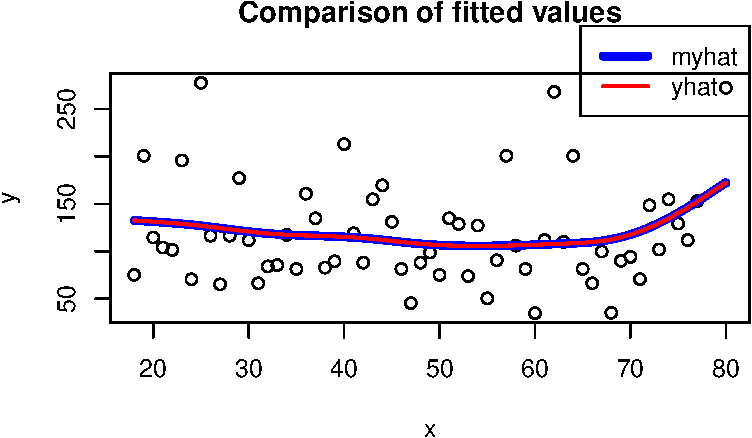
\includegraphics[width=0.8\linewidth]{3LinReg_files/figure-beamer/unnamed-chunk-6-1} \end{center}

\normalsize

\begin{itemize}
\tightlist
\item
  The \(t\)-distribution has heavier tails than the normal distribution.
\item
  For df \(\geq 30\) the \(t\) and Normal distribution are pretty
  similar.
\end{itemize}

\end{block}

\end{frame}

\begin{frame}[fragile]

\begin{block}{Hypothesis tests for bodyfat example}

\(~\)

So let's again go back to the bodyfat regression output:

\vspace{2mm}

\scriptsize

\begin{Shaded}
\begin{Highlighting}[]
\KeywordTok{summary}\NormalTok{(r.bodyfat)}\OperatorTok{$}\NormalTok{coef}
\end{Highlighting}
\end{Shaded}

\begin{verbatim}
##               Estimate Std. Error   t value     Pr(>|t|)
## (Intercept) -26.984368  2.7689004 -9.745518 3.921511e-19
## bmi           1.818778  0.1083411 16.787522 2.063854e-42
\end{verbatim}

\vspace{2mm}

\normalsize

\textbf{Q}: Check how the \texttt{Estimate}, \texttt{Std.\ Error} and
\texttt{t\ value} relate.

\(~\)

\begin{itemize}
\item
  The last column contains the \emph{\(p\)-values} of the tests with
  \(H_0\): \(\beta_0=0\) and \(\beta_1=0\), respectively.
\item
  The \(p\)-value for \texttt{bmi} is very small (\(p<0.0001\)).
  \textbf{What does this mean?}
\end{itemize}

\end{block}

\end{frame}

\begin{frame}

\begin{block}{Recap: Formal definition of the \(p\)-value}

\(~\)

\textbf{The \(p\)-value is} the probability to observe a data summary
(e.g., an average) that is at least as extreme as the one observed,
given that the Null Hypothesis is correct.

\vspace{3mm}

\textbf{Example} (normal distribution): Assume the observed
test-statistic leads to a \(z\)-value = -1.96 \(\Rightarrow\)
\(\text{P}(|z|\geq 1.96)=0.05\) and \(\text{P}(z\leq-1.96)=0.025\) .

\vspace{1mm}

\begin{center}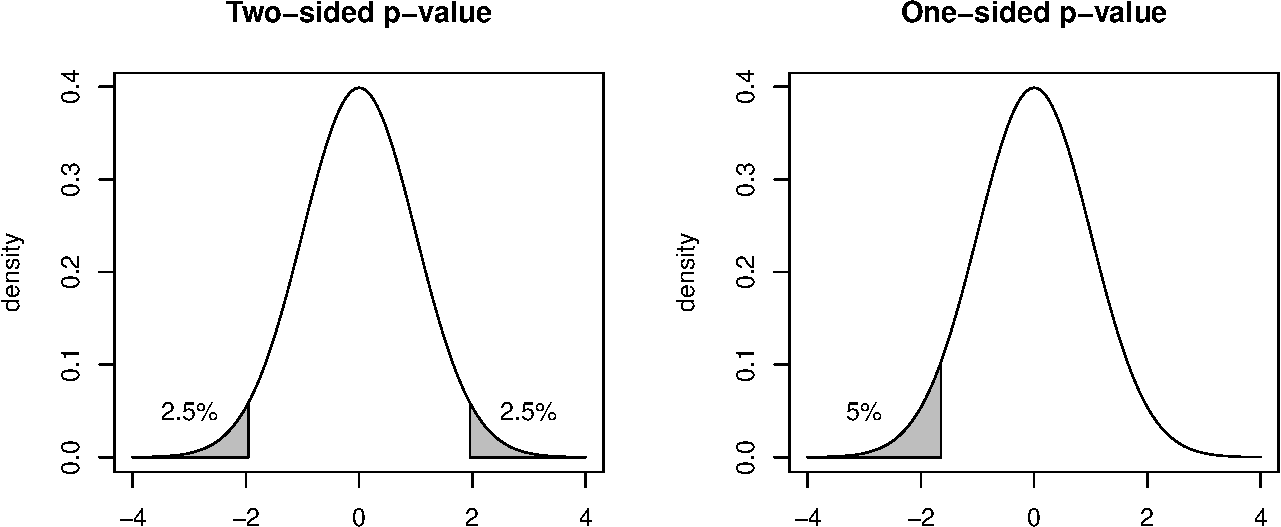
\includegraphics[width=1\linewidth]{3LinReg_files/figure-beamer/pValFig-1} \end{center}

\end{block}

\end{frame}

\begin{frame}

\begin{block}{Recap: Two types of errors}

\vspace{2mm}

In the testing setup, we typically \emph{reject the null hypothesis} if
the \(p\)-value is small enough. Typical cutoffs for the
\emph{significance level} (\(\alpha\)) are \(5\%\) or \(1\%\).

\vspace{2mm}

However, this means we can make two types of errors: \vspace{2mm}

\begin{itemize}
\item
  Type I error:
\item
  Type II error:
\end{itemize}

\vspace{2mm}

\end{block}

\end{frame}

\begin{frame}

\begin{block}{Cautionary notes regarding \(p\)-values:}

\(~\)

\begin{itemize}
\item
  The (mis)use of \(p\)-values is heavily under critique in the
  scientific world!
\item
  Simple yes/no decisions do often stand on very wiggly scientific
  ground.
\end{itemize}

\vspace{2mm}

\(~\)

\scriptsize

We will discuss this a bit in the final module 12. The topic is
connected to good/bad research practice, problems with
``reproducibility'' and scientific progress in general. See e.g.~here:

\begin{itemize}
\tightlist
\item
  The \(p\)-value statement by ASA:
  \url{https://amstat.tandfonline.com/doi/full/10.1080/00031305.2016.1154108\#.Xh16iuExnhM}
\item
  Ideas to redefine what ``statistical significane'' means:
  \url{https://www.nature.com/articles/s41562-017-0189-z}
\item
  A blog by the Scientific American:
  \url{https://blogs.scientificamerican.com/observations/to-fix-the-reproducibility-crisis-rethink-how-we-do-experiments/}
\end{itemize}

\end{block}

\end{frame}

\begin{frame}

\begin{block}{Confidence intervals}

\vspace{2mm}

\begin{itemize}
\tightlist
\item
  Confidence intervals (CIs) are a much more informative way to report
  results than \(p\)-values!
\end{itemize}

\vspace{1mm}

\begin{itemize}
\tightlist
\item
  The
  \(t\)-distribution\footnote{If $n$ is large, the normal approximation to the $t$-distribution can be used (and is used in the textbook).}
  can be used to create confidence intervals for the regression
  parameters. The lower and upper limits of a 95\% confidence interval
  for \(\beta_j\) are
  \[\hat{\beta}_j \pm t_{(1-\alpha/2),n-2} \cdot\text{SE} (\hat{\beta}_j) \quad j=0, 1.\]
\end{itemize}

\vspace{1mm}

\begin{itemize}
\item
  Interpretation of this confidence interval:

  \begin{itemize}
  \item
    There is a 95\% probability that the interval will contain the
    \emph{true} value of \(\beta_j\).
  \item
    \textbf{It is the range of parameter estimates that are
    \emph{compatible with the data} }.
  \end{itemize}
\end{itemize}

\end{block}

\end{frame}

\begin{frame}[fragile]

We can directly ask R to give us the CIs:

\vspace{4mm}

\scriptsize

\begin{Shaded}
\begin{Highlighting}[]
\KeywordTok{confint}\NormalTok{(r.bodyfat, }\DataTypeTok{level =} \KeywordTok{c}\NormalTok{(}\FloatTok{0.95}\NormalTok{))}
\end{Highlighting}
\end{Shaded}

\begin{verbatim}
##                  2.5 %     97.5 %
## (Intercept) -32.438703 -21.530032
## bmi           1.605362   2.032195
\end{verbatim}

\vspace{4mm}

\normalsize

\textbf{Interpretation:}

For an increase in the bmi by one index point, roughly \(\ldots\)
percentage points more bodyfat are expected, and all true values for
\(\beta_1\) between \(\ldots\) and \(\ldots\) are \(\ldots\).

\end{frame}

\begin{frame}{Model accuracy}
\protect\hypertarget{model-accuracy}{}

Measured by

\begin{enumerate}
\tightlist
\item
  The \textbf{residual standard error (RSE)}, which provides an
  \textbf{absolute measure} of \emph{lack of fit} (see above).
\end{enumerate}

\vspace{2mm}

\begin{enumerate}
\setcounter{enumi}{1}
\tightlist
\item
  The \textbf{coefficient of determination \(R^2\)}, which measures the
  proportion of \(y\)'s variance explained by the model (between 0 and
  1), is a \textbf{relative measure} of \emph{lack of fit}:
\end{enumerate}

\[R^2 = \frac{\text{TSS}-\text{RSS}}{\text{TSS}}= 1-\frac{\text{RSS}}{\text{TSS}}=1-\frac{\sum_{i=1}^n(y_i-\hat{y}_i)^2}{\sum_{i=1}^n(y_i-\bar{y}_i)^2}, \]

where \[\text{TSS} = \sum_{i=1}^n (y_i - \bar{y})^2\] is the \emph{total
sum of squares}, a measure for the total variability in \(Y\).

\end{frame}

\begin{frame}[fragile]

\begin{block}{\(R^2\) in simple linear regression}

\vspace{3mm}

\textbf{Note}: In simple linear regression, \(R^2\) is the squared
correlation between the independent and the dependent variable.

\vspace{6mm}

Verify this by comparing \(R^2\) from the bodyfat output to the squared
correlation between the two variables:

\(~\)

\scriptsize

\begin{Shaded}
\begin{Highlighting}[]
\KeywordTok{summary}\NormalTok{(r.bodyfat)}\OperatorTok{$}\NormalTok{r.squared}
\end{Highlighting}
\end{Shaded}

\begin{verbatim}
## [1] 0.5390391
\end{verbatim}

\begin{Shaded}
\begin{Highlighting}[]
\KeywordTok{cor}\NormalTok{(d.bodyfat}\OperatorTok{$}\NormalTok{bodyfat, d.bodyfat}\OperatorTok{$}\NormalTok{bmi)}\OperatorTok{^}\DecValTok{2}
\end{Highlighting}
\end{Shaded}

\begin{verbatim}
## [1] 0.5390391
\end{verbatim}

\end{block}

\end{frame}

\begin{frame}[fragile]{Multiple Linear Regression}
\protect\hypertarget{multiple-linear-regression}{}

Remember that the bodyfat dataset contained much more information than
only bmi and bodyfat:

\begin{itemize}
\tightlist
\item
  \texttt{bodyfat}: \% of body fat.
\item
  \texttt{age}: age of the person.
\item
  \texttt{weight}: body weighth.
\item
  \texttt{height}: body height.
\item
  \texttt{bmi}: bmi.
\item
  \texttt{abdomen}: circumference of abdomen.
\item
  \texttt{hip}: circumference of hip.
\end{itemize}

\end{frame}

\begin{frame}

\begin{block}{Model}

\(~\)

We assume \begin{equation}
Y = \beta_0 + \beta_{1}  X_1 + \beta_2 X_1 + ... + \beta_p X_p + \varepsilon \ ,
\end{equation}

where \(X_j\) is the \(j\)th predictor and \(\beta_j\) the respective
regression coeffficient.

\(~\)

Assume we have \(n\) sampling units \((x_{1i},\ldots,x_{pi}, y_i)\),
\(1\leq i \leq n\), such that each represent an instance of equation
(3), we can use the data matrix

\[{\bf{X}} = \left[\begin{matrix} 1 & x_{11} & ... & x_{1p} \\
1 & x_{21} & ... & x_{2p} \\
\vdots  & ... & ... & \vdots \\
1 & x_{n1} & ... & x_{np} \\
\end{matrix}\right]\]

to write the model in matrix form:
\[{\bf Y}={\bf {X}} \boldsymbol{\beta}+{\boldsymbol{\varepsilon}} \]

\end{block}

\end{frame}

\begin{frame}

\begin{block}{Notation}

\(~\)

\begin{itemize}
\tightlist
\item
  \({\bf Y}: (n \times 1)\) vector of responses (e.g., bodyfat).
\end{itemize}

\vspace{2mm}

\begin{itemize}
\tightlist
\item
  \({\bf X}: (n \times (p+1))\) design matrix, and
  \({\boldsymbol x}_i^T\) is a \((p+1)\)-dimensional row vector for
  observation \(i\).
\end{itemize}

\vspace{2mm}

\begin{itemize}
\tightlist
\item
  \({\boldsymbol \beta}: ((p+1) \times 1)\) vector of regression
  parameters \((\beta_0,\beta_1,\ldots,\beta_p)^\top\).
\end{itemize}

\vspace{2mm}

\begin{itemize}
\tightlist
\item
  \({\boldsymbol \varepsilon}: (n\times 1)\) vector of random errors.
\end{itemize}

\vspace{2mm}

\begin{itemize}
\tightlist
\item
  We assume that pairs \(({\boldsymbol x}_i^T,y_i)\) \((i=1,...,n)\) are
  measured from \emph{independent} sampling units.
\end{itemize}

\(~\)

Remark: other books, including the book in TMA4267 and TMA4315 define
\(p\) to include the intercept. This may lead to some confusion about
\(p\) or \(p+1\) in formulas\ldots{}

\end{block}

\end{frame}

\begin{frame}

\begin{block}{Classical linear model}

\(~\)

\[{\bf Y=X \boldsymbol\beta}+{\boldsymbol \varepsilon}\]

Assumptions: \vspace{2mm}

\begin{enumerate}
\tightlist
\item
  \(\mathsf{E}(\boldsymbol{\varepsilon})=\boldsymbol{0}\). \vspace{2mm}
\item
  \(\mathsf{Cov}(\boldsymbol{\varepsilon})=\mathsf{E}(\boldsymbol{\varepsilon}\boldsymbol{\varepsilon}^T)=\sigma^2\boldsymbol{I}\).
  \vspace{2mm}
\item
  The design matrix has full rank, \(\text{rank}({\bf X})=p+1\). (We
  assume \(n>>(p+1)\).)
\end{enumerate}

\vspace{2mm}

The classical \emph{normal} linear regression model is obtained if
additionally

\begin{enumerate}
\setcounter{enumi}{3}
\tightlist
\item
  \(\boldsymbol\varepsilon\sim N_n({\boldsymbol 0},\sigma^2 {\bf I})\)
  holds. Here \(N_n\) denotes the \(n\)-dimensional multivarate normal
  distribution.
\end{enumerate}

\end{block}

\end{frame}

\begin{frame}[fragile]

\begin{block}{The bodyfat example for two predictors}

\(~\)

We are looking at the regression model

\begin{equation*}
Y = \beta_0 + \beta_{1}  X_1 + \beta_2 X_1  + \varepsilon \ ,
\end{equation*}

with bodyfat as the response (\(Y\)) and \texttt{bmi} and \texttt{age}
as \(X_1\) and \(X_2\).

\(~\)

\normalsize

The regression

\scriptsize

\begin{Shaded}
\begin{Highlighting}[]
\NormalTok{r.bodyfat =}\StringTok{ }\KeywordTok{lm}\NormalTok{(bodyfat }\OperatorTok{~}\StringTok{ }\NormalTok{bmi }\OperatorTok{+}\StringTok{ }\NormalTok{age, }\DataTypeTok{data =}\NormalTok{ d.bodyfat)}
\end{Highlighting}
\end{Shaded}

\(~\)

\normalsize

The \emph{\textcolor{red}{design matrix}}:

\scriptsize

\begin{Shaded}
\begin{Highlighting}[]
\KeywordTok{head}\NormalTok{(}\KeywordTok{model.matrix}\NormalTok{(r.bodyfat))}
\end{Highlighting}
\end{Shaded}

\begin{verbatim}
##   (Intercept)   bmi age
## 1           1 23.65  23
## 2           1 23.36  22
## 3           1 24.69  22
## 4           1 24.91  26
## 5           1 25.54  24
## 6           1 26.48  24
\end{verbatim}

\normalsize

\end{block}

\end{frame}

\begin{frame}

\begin{block}{Distribution of the response vector}

\(~\)

Assume that

\[{\bf Y=X \boldsymbol\beta}+{\boldsymbol \varepsilon} \ , \quad \boldsymbol\varepsilon\sim N_n({\bf 0},\sigma^2 {\bf I}) \ . \]

\vspace{4mm}

\textbf{Q:}

\begin{itemize}
\item
  What is the mean \(\mathsf{E}(\bf Y)\)?
\item
  The covariance matrix \(\mathsf{Cov}(\bf Y)\) given \(\bf{X}\)?
\item
  Thus what is the distribution of \(\bf Y\)?
\end{itemize}

\end{block}

\end{frame}

\begin{frame}

\textbf{A}:
\[ {\bf Y} \sim N_{n}({\bf X} {\boldsymbol\beta},\sigma^2 {\bf I})\]

\end{frame}

\begin{frame}

\begin{block}{Parameter estimation for \(\boldsymbol{\beta}\)}

\(~\)

In multiple linear regression, the parameter vector \(\boldsymbol\beta\)
is estimated with \emph{\textcolor{red}{maximum likelihood}} and
\emph{\textcolor{red}{least squares}}. These two methods give the same
estimator when we assume the normal linear regression model.

\(~\)

With least suqres, we minimize the RSS for a multiple linear regression
model:
\[\begin{aligned} \text{RSS} &=\sum_{i=1}^n (y_i - \hat y_i)^2 = \sum_{i=1}^n (y_i - \hat \beta_0 - \hat \beta_1 x_{i1} - \hat \beta_2 x_{i2} -...-\hat \beta_p x_{ip} )^2 \\
&= \sum_{i=1}^n (y_i-{\boldsymbol x}_i^T \hat{\boldsymbol\beta})^2=({\bf Y}-{\bf X}\hat{\boldsymbol{\beta}})^T({\bf Y}-{\bf X}\hat{\boldsymbol{\beta}})\end{aligned}\]
The estimator is found by solving the system of \((p+1)\) equations

\[\frac{\partial \text{RSS}}{\partial \boldsymbol \beta}={\bf 0} \ .\]

\(\rightarrow\) Derivation on the board.

\end{block}

\end{frame}

\begin{frame}

Summing up:

\textbf{The least squares and maximum likelihood estimator for ${\boldsymbol \beta}$:}
is given like
\[ \hat{\boldsymbol\beta}=({\bf X}^T{\bf X})^{-1} {\bf X}^T {\bf Y} \ .\]

\end{frame}

\begin{frame}[fragile]

\begin{block}{Example continued}

\vspace{5mm}

\tiny

\begin{Shaded}
\begin{Highlighting}[]
\NormalTok{r.bodyfat3 <-}\StringTok{ }\KeywordTok{lm}\NormalTok{(bodyfat }\OperatorTok{~}\StringTok{ }\NormalTok{bmi }\OperatorTok{+}\StringTok{ }\NormalTok{age }\OperatorTok{+}\StringTok{ }\NormalTok{neck }\OperatorTok{+}\StringTok{ }\NormalTok{hip }\OperatorTok{+}\StringTok{ }\NormalTok{abdomen, }\DataTypeTok{data =}\NormalTok{ d.bodyfat)}
\KeywordTok{summary}\NormalTok{(r.bodyfat3)}
\end{Highlighting}
\end{Shaded}

\begin{verbatim}
## 
## Call:
## lm(formula = bodyfat ~ bmi + age + neck + hip + abdomen, data = d.bodyfat)
## 
## Residuals:
##     Min      1Q  Median      3Q     Max 
## -9.3727 -3.1884 -0.1559  3.1003 12.7613 
## 
## Coefficients:
##             Estimate Std. Error t value Pr(>|t|)    
## (Intercept) -7.74965    7.29830  -1.062  0.28939    
## bmi          0.42647    0.23133   1.844  0.06649 .  
## age          0.01457    0.02783   0.524  0.60100    
## neck        -0.80206    0.19097  -4.200 3.78e-05 ***
## hip         -0.31764    0.10751  -2.954  0.00345 ** 
## abdomen      0.83909    0.08418   9.968  < 2e-16 ***
## ---
## Signif. codes:  0 '***' 0.001 '**' 0.01 '*' 0.05 '.' 0.1 ' ' 1
## 
## Residual standard error: 4.392 on 237 degrees of freedom
## Multiple R-squared:  0.7185, Adjusted R-squared:  0.7126 
## F-statistic:   121 on 5 and 237 DF,  p-value: < 2.2e-16
\end{verbatim}

\normalsize

\end{block}

\end{frame}

\begin{frame}[fragile]

Reproduce the values under \texttt{Estimate} by calculating without the
use of \texttt{lm}.

\(~\)

\scriptsize

\begin{Shaded}
\begin{Highlighting}[]
\NormalTok{X =}\StringTok{ }\KeywordTok{model.matrix}\NormalTok{(r.bodyfat3)}
\NormalTok{Y =}\StringTok{ }\NormalTok{d.bodyfat}\OperatorTok{$}\NormalTok{bodyfat}
\NormalTok{betahat =}\StringTok{ }\KeywordTok{solve}\NormalTok{(}\KeywordTok{t}\NormalTok{(X) }\OperatorTok\StringTok{ }\NormalTok{X) }\OperatorTok\StringTok{ }\KeywordTok{t}\NormalTok{(X) }\OperatorTok\StringTok{ }\NormalTok{Y}
\KeywordTok{print}\NormalTok{(betahat)}
\end{Highlighting}
\end{Shaded}

\begin{verbatim}
##                    [,1]
## (Intercept) -7.74964673
## bmi          0.42647368
## age          0.01457356
## neck        -0.80206081
## hip         -0.31764315
## abdomen      0.83909391
\end{verbatim}

\end{frame}

\begin{frame}

\begin{block}{Distribution of the regression parameter estimator}

\vspace{2mm}

Given
\[ \hat{\boldsymbol\beta}=({\bf X}^T{\bf X})^{-1} {\bf X}^T {\bf Y} \ ,\]

\textbf{what are}

\begin{itemize}
\tightlist
\item
  The mean \(\mathsf{E}(\hat{\boldsymbol\beta})\)?
\item
  The covariance matrix \(\mathsf{Cov}(\hat{\boldsymbol\beta})\)?
\item
  The distribution of \(\hat{\boldsymbol\beta}\)?
\end{itemize}

\vspace{4mm}

\textbf{Hint:} Use that

\begin{itemize}
\tightlist
\item
  \(\hat{\boldsymbol\beta}={\bf C}{\bf Y}\) with
  \({\bf C}=({\bf X}^T{\bf X})^{-1} {\bf X}^T\).
\item
  \({\bf Y} \sim N_{n}({\bf X} {\boldsymbol\beta},\sigma^2 {\bf I})\).
\end{itemize}

\end{block}

\end{frame}

\begin{frame}

\textbf{Answers:}

See Problem 3 of recommended exercise 3 (and the respective solutions)
to derive that

\[\hat{\boldsymbol\beta}\sim N_{p+1}(\boldsymbol{\beta},\underbrace{\sigma^2({\bf X}^T{\bf X})^{-1}}_{\text{covariance matrix}}) \ . \]

\end{frame}

\begin{frame}[fragile]

\begin{block}{The covariance matrix of \(\boldsymbol{\hat\beta}\) in R}

\(~\)

The covariance matrix for the \(\boldsymbol{\hat\beta}\) can be obtained
as follows:

\(~\)

\scriptsize

\begin{Shaded}
\begin{Highlighting}[]
\KeywordTok{vcov}\NormalTok{(r.bodyfat3)}
\end{Highlighting}
\end{Shaded}

\begin{verbatim}
##             (Intercept)           bmi           age          neck
## (Intercept) 53.26521684  0.6774596810 -0.0780438125 -0.7219656479
## bmi          0.67745968  0.0535131152  0.0005729015 -0.0120408637
## age         -0.07804381  0.0005729015  0.0007745054 -0.0003432518
## neck        -0.72196565 -0.0120408637 -0.0003432518  0.0364680351
## hip         -0.54820573 -0.0058040729  0.0015239515 -0.0027159299
## abdomen      0.16457979 -0.0110809165 -0.0011917596 -0.0007706161
##                      hip       abdomen
## (Intercept) -0.548205733  0.1645797895
## bmi         -0.005804073 -0.0110809165
## age          0.001523951 -0.0011917596
## neck        -0.002715930 -0.0007706161
## hip          0.011558850 -0.0045707222
## abdomen     -0.004570722  0.0070861066
\end{verbatim}

\end{block}

\end{frame}

\begin{frame}

How does this compare to simple linear regression? Not so easy to see a
connection!

\[\hat{\beta}_0 = \bar{Y}-\hat{\beta}_1 \bar{x} \text{ and } \hat{\beta}_1 = \frac{\sum_{i=1}^n(x_i-\bar{x})(Y_i-\bar{Y})}{\sum_{i=1}^n(x_i-\bar{x})^2},\]

\[ \hat{\boldsymbol\beta}=({\bf X}^T{\bf X})^{-1} {\bf X}^T {\bf Y} \ .\]

\(~\)

\textbf{Exercise:} Verify the connection using
\(\boldsymbol\beta=(\beta_0,\beta_1)^\top\) and
\({\bf X}= \left[\begin{matrix} 1 & x_{11} \\ 1 & x_{21} \\ 1 & \vdots \\ 1 & x_{n1} \\ \end{matrix}\right]\).

\end{frame}

\begin{frame}{Four important questions}
\protect\hypertarget{four-important-questions}{}

\begin{enumerate}
\item
  Is at least one of the predictors \(X_1, \ldots, X_p\) useful in
  predicting the response?
\item
  Do all the predictors help to explain \(Y\), or is only a subset of
  predictors useful?
\item
  How well does the model fit the data?
\item
  Given a set of predictor variables, what response value should we
  predict, and how accurate is our prediction?
\end{enumerate}

\end{frame}

\begin{frame}

\begin{block}{1. Relationship between predictors and response?}

\(~\)

Question is whether we could as well omit all predictor variables at the
same time, that is

\begin{center}
$$H_0: \beta_1=\beta_2=\ldots=\beta_p=0 $$

vs. 
$$H_1: \text{at least one } \beta_j \text{ is non-zero.}$$
\end{center}

\end{block}

\end{frame}

\begin{frame}

\vspace{4mm}

To answer this, we need the \(F\)-statistic

\[F = \frac{(\text{TSS}-\text{RSS})/p}{\text{RSS}/(n-p-1)} \sim F_{p,(n-p-1)}\ ,\]

where total sum of squares \(\text{TSS}=\sum_i(y_i-\bar{y})^2\), and
residual sum of squares \(\text{RSS}=\sum_i(y_i-\hat{y}_i)^2\). Under
the Normal regression assumptions, \(F\) follows an \(F_{p,(n-p-1)}\)
distribution (see Walepole et al. (2012), Chapter 8.7).

\begin{itemize}
\item
  If \(H_0\) is true, \(F\) is expected to be \(\approx 1\).
\item
  Otherwise, we expect that the numerator is larger than the denominator
  (because the regression then explains a lot of variation) and thus
  \(F\) is greater than 1. For an observed value \(f_0\), the
  \(p\)-value is given as \[p =P(F_{p,n-p-1}> f_0) \ .\]
\end{itemize}

\end{frame}

\begin{frame}[fragile]

Checking the \(F\)-value in the \texttt{R} output:

\(~\)

\scriptsize

\begin{Shaded}
\begin{Highlighting}[]
\KeywordTok{summary}\NormalTok{(r.bodyfat)}
\end{Highlighting}
\end{Shaded}

\begin{verbatim}
## 
## Call:
## lm(formula = bodyfat ~ bmi + age, data = d.bodyfat)
## 
## Residuals:
##      Min       1Q   Median       3Q      Max 
## -12.0415  -3.8725  -0.1237   3.9193  12.6599 
## 
## Coefficients:
##              Estimate Std. Error t value Pr(>|t|)    
## (Intercept) -31.25451    2.78973 -11.203  < 2e-16 ***
## bmi           1.75257    0.10449  16.773  < 2e-16 ***
## age           0.13268    0.02732   4.857 2.15e-06 ***
## ---
## Signif. codes:  0 '***' 0.001 '**' 0.01 '*' 0.05 '.' 0.1 ' ' 1
## 
## Residual standard error: 5.329 on 240 degrees of freedom
## Multiple R-squared:  0.5803, Adjusted R-squared:  0.5768 
## F-statistic: 165.9 on 2 and 240 DF,  p-value: < 2.2e-16
\end{verbatim}

\(~\)

\normalsize

Conclusion?

\end{frame}

\begin{frame}

\begin{block}{More complex hypotheses}

\(~\)

Sometimes we don't want to test if all \(\beta\)'s are zero at the same
time, but only a subset \(1,\ldots , q\):

\[ H_0: \beta_1=\beta_2=\cdots= \beta_q =0\] \text{  vs.  }
\[H_1: \text{at least one different from zero}.\]

\vspace{2mm}

Again, the \(F\)-test can be used, but now \(F\) is calculated like

\[F=\frac{(\text{RSS$_0$-RSS})/(q)}{\text{RSS}/(n-p-1)} \sim F_{q,n-p-1} \ ,\]

where

\begin{itemize}
\tightlist
\item
  Large model: RSS with \(p+1\) regression parameters
\item
  Small model: RSS\(_0\) with \(q+1\) regression parameters
\end{itemize}

\end{block}

\end{frame}

\begin{frame}[fragile]

\begin{block}{Example in R}

\vspace{3mm}

\begin{itemize}
\item
  \textbf{Question:} Do \texttt{weight} and \texttt{height} explain
  something of \texttt{bodyfat}, on top of the variables \texttt{bmi}
  and \texttt{age}?
\item
  Fit both models and use the \texttt{anova()} function to carry out the
  \(F\)-test:
\end{itemize}

\(~\)

\footnotesize

\begin{Shaded}
\begin{Highlighting}[]
\NormalTok{r.bodyfat.small =}\StringTok{ }\KeywordTok{lm}\NormalTok{(bodyfat }\OperatorTok{~}\StringTok{ }\NormalTok{bmi }\OperatorTok{+}\StringTok{ }\NormalTok{age, }\DataTypeTok{data =}\NormalTok{ d.bodyfat)}
\NormalTok{r.bodyfat.large =}\StringTok{ }\KeywordTok{lm}\NormalTok{(bodyfat }\OperatorTok{~}\StringTok{ }\NormalTok{bmi }\OperatorTok{+}\StringTok{ }\NormalTok{age }\OperatorTok{+}\StringTok{ }\NormalTok{weight }\OperatorTok{+}\StringTok{ }\NormalTok{height, }\DataTypeTok{data =}\NormalTok{ d.bodyfat)}
\KeywordTok{anova}\NormalTok{(r.bodyfat.small, r.bodyfat.large)}
\end{Highlighting}
\end{Shaded}

\begin{verbatim}
## Analysis of Variance Table
## 
## Model 1: bodyfat ~ bmi + age
## Model 2: bodyfat ~ bmi + age + weight + height
##   Res.Df    RSS Df Sum of Sq      F Pr(>F)
## 1    240 6816.2                           
## 2    238 6702.9  2    113.28 2.0112 0.1361
\end{verbatim}

\normalsize

\end{block}

\end{frame}

\begin{frame}

\begin{block}{Inference about a single predictor \(\beta_j\)}

\(~\)

A special case is

\[H_0: \beta_j=0 \; \text{ vs. } \; H_1: \beta_j\neq 0\] \vspace{2mm}

\begin{itemize}
\item
  Nothing new: We did it for simple linear regression!
\item
  This makes sense: it is known that (or you can try to show it
  yourself) \[F_{1,n-p-1} = t^2_{n-p-1} \ ,\] thus we can use a
  \(T\)-statistics with \((n-p-1)\) degrees of freedom to get the
  \(p\)-value.
\end{itemize}

\end{block}

\end{frame}

\begin{frame}[fragile]

Going back again:

\(~\)

\footnotesize

\begin{Shaded}
\begin{Highlighting}[]
\KeywordTok{summary}\NormalTok{(r.bodyfat)}\OperatorTok{$}\NormalTok{coef}
\end{Highlighting}
\end{Shaded}

\begin{verbatim}
##                Estimate Std. Error    t value     Pr(>|t|)
## (Intercept) -31.2545057 2.78973238 -11.203406 1.039096e-23
## bmi           1.7525705 0.10448723  16.773060 2.600646e-42
## age           0.1326767 0.02731582   4.857137 2.149482e-06
\end{verbatim}

\normalsize

\(~\)

\textbf{However}:

\begin{itemize}
\item
  Only checking the individual \(p\)-values is dangerous.
  \textbf{Why?}\\
\item
  Not possible if \(n>p\) \(\rightarrow\) need other approaches (see
  e.g., Module 6).
\end{itemize}

\end{frame}

\begin{frame}[fragile]

\begin{block}{Inference about \(\beta_j\): confidence interval}

\(~\)

\begin{itemize}
\tightlist
\item
  Using that
  \[ T_j=\frac{\hat{\beta}_j}{\text{SE}(\hat\beta_j)}\sim t_{n-p-1} \ ,\]
  we can create confidence intervals for \(\beta_j\) in the same manner
  as we did for simple linear regression (see slide 41). For example,
  when using the typical confidence level \(\alpha=0.05\) we have
\end{itemize}

\[\hat{\beta}_j \pm t_{0.975,n-p-2} \cdot\text{SE} (\hat{\beta}_j)  \ .\]

\vspace{4mm}

\footnotesize

\begin{Shaded}
\begin{Highlighting}[]
\KeywordTok{confint}\NormalTok{(r.bodyfat)}
\end{Highlighting}
\end{Shaded}

\begin{verbatim}
##                   2.5 %      97.5 %
## (Intercept) -36.7499929 -25.7590185
## bmi           1.5467413   1.9583996
## age           0.0788673   0.1864861
\end{verbatim}

\end{block}

\end{frame}

\begin{frame}

\begin{block}{2. Deciding on important variables}

\(~\)

Overarching question:

\(~\)

\begin{center}
 \emph{\textcolor{blue}{\bf Which model is the best?}}
\end{center}

\vspace{2mm}

But:

\begin{itemize}
\item
  Not clear what \emph{best} means \(\rightarrow\) we need an objective
  criterion, like AIC, BIC, Mallows \(C_p\), adjusted \(R^2\).
\item
  There are usually \textbf{many} possible models. For \(p\) predictors,
  we can build \(2^p\) different models.
\item
  \textbf{Cautionary note}: Model selection can also lead to biased
  parameters estimates.
\end{itemize}

\(~\)

\(\rightarrow\) This topic is the focus of Module 6.

\end{block}

\end{frame}

\begin{frame}

\begin{block}{3. Model Fit}

\(~\)

We can again look at the two measures from simple linear regression:

\(~\)

\begin{itemize}
\tightlist
\item
  An absolute measure of lack of fit is again given by the estimate of
  \(\sigma\), the residual standard error (RSE)
\end{itemize}

\[\hat\sigma = \text{RSE}= \sqrt{ \frac{ \text{RSS}}{n-p-1}} \ . \]

\begin{itemize}
\tightlist
\item
  \(R^2\) is again the fraction of variance explained (no change from
  simple linear regression)
  \[R^2 = \frac{\text{TSS}-\text{RSS}}{\text{TSS}}= 1-\frac{\text{RSS}}{\text{TSS}}=1-\frac{\sum_{i=1}^n(y_i-\hat{y}_i)^2}{\sum_{i=1}^n(y_i-\bar{y}_i)^2} \ .\]
  Simply speaking: ``The higher \(R^2\), the better.''
\end{itemize}

\end{block}

\end{frame}

\begin{frame}[fragile]

\begin{block}{However: Caveat with \(R^2\)}

\(~\)

Let us look at the \(R^2\)s from the three bodyfat models

\vspace{2mm}

model 1: \(y\sim bmi\)

model 2: \(y\sim bmi + age\)

model 3: \(y\sim bmi + age + neck + hip + abdomen\)

\(~\)

\tiny

\begin{Shaded}
\begin{Highlighting}[]
\KeywordTok{summary}\NormalTok{(r.bodyfatM1)}\OperatorTok{$}\NormalTok{r.squared}
\end{Highlighting}
\end{Shaded}

\begin{verbatim}
## [1] 0.5390391
\end{verbatim}

\begin{Shaded}
\begin{Highlighting}[]
\KeywordTok{summary}\NormalTok{(r.bodyfatM2)}\OperatorTok{$}\NormalTok{r.squared}
\end{Highlighting}
\end{Shaded}

\begin{verbatim}
## [1] 0.5802956
\end{verbatim}

\begin{Shaded}
\begin{Highlighting}[]
\KeywordTok{summary}\NormalTok{(r.bodyfatM3)}\OperatorTok{$}\NormalTok{r.squared}
\end{Highlighting}
\end{Shaded}

\begin{verbatim}
## [1] 0.718497
\end{verbatim}

\(~\)

\normalsize

The models explain 54\%, 58\% and 72\% of the total variability of
\(y\).

It thus \emph{seems} that larger models are ``better''. However, \(R^2\)
does always increase when new variables are included, but this does not
mean that the model is more reasonable.

\end{block}

\end{frame}

\begin{frame}

\begin{block}{Adjusted \(R^2\)}

\(~\)

When the sample size \(n\) is small with respect to the number of
variables \(m\) included in the model, an \emph{adjusted} \(R^2\) gives
a better (``fairer'') estimation of the actual variability that is
explained by the covariates:

\begin{equation*}
R^2_a = 1-(1-R^2 )\frac{n-1}{n-m-1}
\end{equation*}

\(~\)

\(R^2_a\) \textbf{penalizes for adding more variables} if they do not
really improve the model!

\(~\)

\(\rightarrow\) \(R_a\) may decrease when a new variable is added.

\end{block}

\end{frame}

\begin{frame}

\begin{block}{Model fit -- in a broader sense}

\(~\)

We will look at model validation / model checking later.

\end{block}

\end{frame}

\begin{frame}

\begin{block}{4. Predictions: Two questions}

\(~\)

\begin{enumerate}
\tightlist
\item
  \textbf{Which other regression lines are compatible with the observed
  data?}
\end{enumerate}

\vspace{2mm}

\(\rightarrow\) We can use \(\hat\beta_0, \ldots , \hat\beta_p\) to
estimate the \emph{least squares plane}
\[\hat{Y} = \hat\beta_0 + \hat\beta_1 X_1 + \ldots + \hat\beta_p X_p \]
as an approximation of
\(f(X) = \beta_0 + \beta_1 X_1 + \ldots + \beta_p X_p .\) This leads to
the \emph{\textcolor{red}{confidence interval}}.

\vspace{4mm}

\begin{enumerate}
\setcounter{enumi}{1}
\tightlist
\item
  \textbf{Where do future observations with a given \(x\) coordinate
  lie?}
\end{enumerate}

\vspace{2mm}

\(\rightarrow\) Even if we could predict \(\hat{Y}=f(X)\), the
\emph{true} value \(Y = f(X) + \varepsilon\) varies around \(\hat{Y}\).
We can compute a \emph{\textcolor{red}{prediction interval}} for new
observations \(Y\).

\end{block}

\end{frame}

\begin{frame}

\begin{center}\includegraphics[width=0.5\linewidth]{3LinReg_files/figure-beamer/unnamed-chunk-22-1} \end{center}

\begin{itemize}
\tightlist
\item
  Plotting the confidence and prediction intervals around all predicted
  values \(\hat Y_0\) one obtains the \textbf{confidence range} or
  \textbf{confidence band} for the expected values of \(Y\).
\end{itemize}

\vspace{2mm}

Note: The prediction range is much broader than the confidence range.
Why?

\end{frame}

\begin{frame}

\begin{block}{Calculation of the confidence intervals/range}

\(~\)

\begin{itemize}
\tightlist
\item
  Given a realization of \(X_1, \ldots ,X_p\), say
  \(x_1^{(0)}, \ldots x_p^{(0)}\). The question is:\\
  \vspace{2mm} \textbf{Where does
  \(\hat y_0 = \hat\beta_0 + \hat\beta_1 x_1^{(0)} + \ldots \hat\beta_p x_p^{(0)}\)
  lie with a certain confidence (i.e., 95\%)?}
\end{itemize}

\vspace{6mm}

\begin{itemize}
\tightlist
\item
  This question is not trivial, because
  \(\hat\beta_0, \ldots \hat\beta_p\) are estimates from the data and
  contain uncertainty.
\end{itemize}

\(~\)

\vspace{4mm}

\begin{itemize}
\tightlist
\item
  For the confidence range, only the uncertainty in the estimates
  \(\hat\beta_0, \ldots \hat\beta_p\) matters.
\end{itemize}

\end{block}

\end{frame}

\begin{frame}

\begin{block}{Calculation of the prediction intervals/range}

\(~\)

\begin{itemize}
\tightlist
\item
  Given a new value of \(X_1, \ldots, X_p\), say
  \(x_1^{(0)}, \ldots x_p^{(0)}\). The question is:\\
  \vspace{2mm} \textbf{Where does a future observation \(y_0\) lie with
  a certain confidence (i.e., 95\%)?}
\end{itemize}

\vspace{6mm}

\begin{itemize}
\item
  To answer this question, we have to sum uncertainty over two
  components:

  \begin{enumerate}
  \item
    the \emph{\textcolor{red}{uncertainty in the predicted value}}
    \(\hat y_0 = \hat\beta_0 + \hat\beta_1 x_1^{(0)} + \ldots \hat\beta_p x_p^{(0)}\)
    (due to uncertainty in \(\hat{\boldsymbol\beta}\)).
  \item
    the \emph{\textcolor{red}{irreducible error}}
    \(\varepsilon_0 \sim N(0,\sigma^2)\).
  \end{enumerate}
\end{itemize}

\vspace{4mm}

\begin{itemize}
\tightlist
\item
  The \emph{prediction intervals and range are always wider than the
  confidence intervals and range}.
\end{itemize}

\end{block}

\end{frame}

\begin{frame}[fragile]

\begin{itemize}
\tightlist
\item
  Confidence and prediction intervals for given data points can be found
  in R using \texttt{predict} on an \texttt{lm} object (make sure that
  \texttt{newdata} is a \texttt{data.frame} with the same names as the
  original data).
\end{itemize}

\(~\)

\scriptsize

\begin{Shaded}
\begin{Highlighting}[]
\NormalTok{fit =}\StringTok{ }\KeywordTok{lm}\NormalTok{(bodyfat }\OperatorTok{~}\StringTok{ }\NormalTok{bmi }\OperatorTok{+}\StringTok{ }\NormalTok{age }\OperatorTok{+}\StringTok{ }\NormalTok{abdomen, }\DataTypeTok{data =}\NormalTok{ d.bodyfat)}
\NormalTok{newobs =}\StringTok{ }\NormalTok{d.bodyfat[}\DecValTok{1}\NormalTok{, ]}
\end{Highlighting}
\end{Shaded}

\begin{Shaded}
\begin{Highlighting}[]
\KeywordTok{predict}\NormalTok{(fit, }\DataTypeTok{newdata =}\NormalTok{ newobs, }\DataTypeTok{interval =} \StringTok{"confidence"}\NormalTok{, }\DataTypeTok{type =} \StringTok{"response"}\NormalTok{)}
\end{Highlighting}
\end{Shaded}

\begin{verbatim}
##        fit      lwr      upr
## 1 13.17595 11.99122 14.36069
\end{verbatim}

\begin{Shaded}
\begin{Highlighting}[]
\KeywordTok{predict}\NormalTok{(fit, }\DataTypeTok{newdata =}\NormalTok{ newobs, }\DataTypeTok{interval =} \StringTok{"prediction"}\NormalTok{, }\DataTypeTok{type =} \StringTok{"response"}\NormalTok{)}
\end{Highlighting}
\end{Shaded}

\begin{verbatim}
##        fit      lwr     upr
## 1 13.17595 3.951613 22.4003
\end{verbatim}

\end{frame}

\begin{frame}

Finally, we need to keep in mind that the model we work with is only an
\emph{approximation of the reality}. In fact,

\vspace{4mm}

In 2014, David Hand wrote:

\vspace{4mm}

\begin{quote}
In general, when building statistical models, we must
not forget that the aim is to understand something about
the real world. Or predict, choose an action, make
a decision, summarize evidence, and so on, but always
about the real world, not an abstract mathematical
world: our models are not the reality -- a point well
made by George Box in his often-cited remark that
``all models are wrong, but some are useful''.
\end{quote}

(Box 1979)

\end{frame}

\begin{frame}{Extensions of the linear model}
\protect\hypertarget{extensions-of-the-linear-model}{}

Extensions that make the linear model very powerful:

\(~\)

\begin{itemize}
\tightlist
\item
  Binary covariates (e.g., male/female, smoker/non-smoker)
\end{itemize}

\vspace{2mm}

\begin{itemize}
\tightlist
\item
  Categorical covariates (e.g., black/white/green)?
\end{itemize}

\vspace{2mm}

\begin{itemize}
\tightlist
\item
  Interaction terms
\end{itemize}

\vspace{2mm}

\begin{itemize}
\tightlist
\item
  Non-linear terms
\end{itemize}

\end{frame}

\begin{frame}

\begin{block}{Binary predictors}

\(~\)

So far, the covariates \(X\) were always continuous.\\
\vspace{2mm}

In reality, there are no restrictions assumed with respect to the \(X\)
variables. \vspace{2mm}

One very frequent data type are \textbf{binary} variables, that is,
variables that can only attain values 0 or 1. \vspace{4mm}

If the binary variable \(x\) is the only variable in the model
\(Y_i = \beta_0 + \beta_1 x_i + \varepsilon_i\), the model has only two
predicted outcomes (plus error):

\begin{equation*}
Y_i = \left\{ 
\begin{array}{ll}
 \beta_0  + \varepsilon_i \quad &\text{if } x_i=0 \ , \\
 \beta_0 + \beta_1 + \varepsilon_i \quad &\text{if } x_i =1 \ .\\
\end{array}
\right .
\end{equation*}

\vspace{4mm}

\textbf{Example}: Credit card data analysis in Section 3.3.1 in the ISLR
book.

\end{block}

\end{frame}

\begin{frame}

\begin{block}{Qualitative predictors with more than 2 levels}

\(~\)

More generally, a covariate may indicate a \textbf{category}, for
instance the species of an animal or a plant. This type of covariate is
called a \textbf{factor}. The trick: convert a factor variable \(X\)
with \(k\) levels (for instance 3 species) into \(k\) dummy variables
\(X_j\) with \vspace{2mm}

\begin{equation*}
x_{ij} = \left\{ 
\begin{array} {ll}
1, & \text{if the $i$th observation belongs to group $j$}.\\
0, & \text{otherwise.}
\end{array}\right.
\end{equation*}

\vspace{4mm}

Each of the covariates \(x_1,\ldots, x_k\) can then be included as a
binary variable in the model \begin{equation*}
y_i = \beta_0 + \beta_1 x_1 + \ldots + \beta_k x_k + \varepsilon_i \ .
\end{equation*}

\vspace{6mm}

However: this model is
\emph{\textcolor{red}{not identifiable}}.\footnote{What does that mean? I could add a constant to $\beta_1, \beta_2, ...\beta_k$ and subtract it from $\beta_0$, and the model would fit equally well to the data, so it cannot be decided which set of the parameters is best.}

\end{block}

\end{frame}

\begin{frame}

\textbf{Solution:} One of the \(k\) categories must be selected as a
\emph{reference category} and is \emph{not included in the model}.
Typically: the first category is the reference, thus \(\beta_1=0\).

\vspace{2mm}

The model thus discriminates between the factor levels, such that
(assuming \(\beta_1=0\))

\begin{equation*}
y_i = \left\{
\begin{array}{ll}
\beta_0 + \varepsilon, & \text{if $x_{i1}=1$ }\\
\beta_0 + \beta_2 + \varepsilon, & \text{if $x_{i2}=1$ }\\
...\\
\beta_0 + \beta_k + \varepsilon, & \text{if $x_{ik}=1$ } \ .
\end{array}\right.
\end{equation*}

\end{frame}

\begin{frame}

\begin{block}{!Important to remember!}

\textcolor{gray}{(Common aspect that leads to confusion!)}

\vspace{10mm}

\emph{\textcolor{red}{A factor covariate with $k$ factor levels requires $k-1$ parameters!}}
\vspace{2mm}

\(\rightarrow\) The \emph{degrees of freedom} of the fitted model are
therefore reduced by \(k-1\).

\end{block}

\end{frame}

\begin{frame}[fragile]

\begin{block}{Example}

\(~\)

We are now using the \texttt{Credit} dataset from the \texttt{ISLR}
library.

\(~\)

\scriptsize

\begin{Shaded}
\begin{Highlighting}[]
\KeywordTok{library}\NormalTok{(ISLR)}
\KeywordTok{data}\NormalTok{(Credit)}
\KeywordTok{head}\NormalTok{(Credit)}
\end{Highlighting}
\end{Shaded}

\begin{verbatim}
##   ID  Income Limit Rating Cards Age Education Gender Student Married
## 1  1  14.891  3606    283     2  34        11   Male      No     Yes
## 2  2 106.025  6645    483     3  82        15 Female     Yes     Yes
## 3  3 104.593  7075    514     4  71        11   Male      No      No
## 4  4 148.924  9504    681     3  36        11 Female      No      No
## 5  5  55.882  4897    357     2  68        16   Male      No     Yes
## 6  6  80.180  8047    569     4  77        10   Male      No      No
##   Ethnicity Balance
## 1 Caucasian     333
## 2     Asian     903
## 3     Asian     580
## 4     Asian     964
## 5 Caucasian     331
## 6 Caucasian    1151
\end{verbatim}

\(~\)

\normalsize

Question: Do the Balances differ for different Ethnicities?

\end{block}

\end{frame}

\begin{frame}[fragile]

\scriptsize

\begin{Shaded}
\begin{Highlighting}[]
\KeywordTok{library}\NormalTok{(GGally)}
\KeywordTok{ggpairs}\NormalTok{(Credit[, }\KeywordTok{c}\NormalTok{(}\DecValTok{2}\NormalTok{, }\DecValTok{6}\NormalTok{, }\DecValTok{11}\NormalTok{, }\DecValTok{12}\NormalTok{)], }\KeywordTok{aes}\NormalTok{(}\DataTypeTok{colour =}\NormalTok{ Ethnicity))}
\end{Highlighting}
\end{Shaded}

\includegraphics[width=0.85\linewidth]{3LinReg_files/figure-beamer/unnamed-chunk-26-1}

\end{frame}

\begin{frame}[fragile]

In R, a factor covariate can be used in the same way as a continuous
predictor:

\(~\)

\scriptsize

\begin{Shaded}
\begin{Highlighting}[]
\NormalTok{r.lm <-}\StringTok{ }\KeywordTok{lm}\NormalTok{(Balance }\OperatorTok{~}\StringTok{ }\NormalTok{Ethnicity, }\DataTypeTok{data =}\NormalTok{ Credit)}
\KeywordTok{summary}\NormalTok{(r.lm)}\OperatorTok{$}\NormalTok{coef}
\end{Highlighting}
\end{Shaded}

\begin{verbatim}
##                     Estimate Std. Error    t value     Pr(>|t|)
## (Intercept)        531.00000   46.31868 11.4640565 1.774117e-26
## EthnicityAsian     -18.68627   65.02107 -0.2873880 7.739652e-01
## EthnicityCaucasian -12.50251   56.68104 -0.2205766 8.255355e-01
\end{verbatim}

\(~\)

\normalsize

Interpretation? Do the ethnicities really differ? Check also the
\(F\)-test in the last line of the summary output.

\(~\)

\begin{equation*}
\hat{y}_i = \left\{
\begin{array}{ll}
\qquad \qquad\qquad \qquad\qquad & \text{if $i$ is Asian}\\[2mm]
\qquad \qquad\qquad \qquad\qquad & \text{if $i$ is Caucasian}\\[2mm]
\qquad \qquad\qquad \qquad\qquad & \text{if $i$ is Afro-American}\\
\end{array}\right.
\end{equation*}

\end{frame}

\begin{frame}[fragile]

\begin{block}{Sidenote: The ``reference category''}

\vspace{2mm}

In the above example we do not see a result for the
\texttt{EthnicityAfrican\ American}. Why?

\begin{itemize}
\tightlist
\item
  \texttt{African\ American} is chosen to be the reference category.
\item
  The results for \texttt{EthnicityAsian} and
  \texttt{EthnicityCaucasian} are \textbf{differences} with respect to
  the reference cateogry.
\item
  R chooses the reference category in alphabetic order! This is
  sometimes not a relevant category.
\item
  You can change the reference category:
\end{itemize}

\(~\)

\scriptsize

\begin{Shaded}
\begin{Highlighting}[]
\KeywordTok{library}\NormalTok{(dplyr)}
\NormalTok{Credit <-}\StringTok{ }\KeywordTok{mutate}\NormalTok{(Credit, }\DataTypeTok{Ethnicity =} \KeywordTok{relevel}\NormalTok{(Ethnicity, }\DataTypeTok{ref =} \StringTok{"Caucasian"}\NormalTok{))}
\NormalTok{r.lm <-}\StringTok{ }\KeywordTok{lm}\NormalTok{(Balance }\OperatorTok{~}\StringTok{ }\NormalTok{Ethnicity, }\DataTypeTok{data =}\NormalTok{ Credit)}
\KeywordTok{summary}\NormalTok{(r.lm)}\OperatorTok{$}\NormalTok{coef}
\end{Highlighting}
\end{Shaded}

\begin{verbatim}
##                             Estimate Std. Error    t value     Pr(>|t|)
## (Intercept)               518.497487   32.66986 15.8708211 2.824537e-44
## EthnicityAfrican American  12.502513   56.68104  0.2205766 8.255355e-01
## EthnicityAsian             -6.183762   56.12165 -0.1101850 9.123184e-01
\end{verbatim}

\vspace{2mm}

\small

Note: The differences are now with respect to the Caucasian category --
the model is however exactly the same!

\end{block}

\end{frame}

\begin{frame}[fragile]

\begin{block}{Testing for a categorical predictor}

\vspace{2mm}

\textbf{Question}: Is a qualitative predictor needed in the model?

\vspace{2mm}

For a predictor with more than two levels (like Ethnicity above), the
Null Hypothesis is whether

\[\beta_1 = \ldots = \beta_{k-1}=0\] at the same time.

\vspace{2mm}

\(\rightarrow\) We again need the
\(F\)-test\footnote{remember that the $F$-test is a generalization of the $t$-test!},
as \textbf{always when we test for more than one \(\beta_j=0\)
\emph{simultaneously}}!

\vspace{2mm}

In R, this is done by the \texttt{anova()} function:

\vspace{2mm}

\scriptsize

\begin{Shaded}
\begin{Highlighting}[]
\KeywordTok{anova}\NormalTok{(r.lm)}
\end{Highlighting}
\end{Shaded}

\begin{verbatim}
## Analysis of Variance Table
## 
## Response: Balance
##            Df   Sum Sq Mean Sq F value Pr(>F)
## Ethnicity   2    18454    9227  0.0434 0.9575
## Residuals 397 84321458  212397
\end{verbatim}

\end{block}

\end{frame}

\begin{frame}[fragile]

\begin{block}{Interactions: Removing the additivity assumption}

\vspace{2mm}

We again look at the \texttt{Credit} dataset. We want to model the
\texttt{Balance} as a function of \texttt{Income} and wheter the person
is a student or not.

\vspace{2mm}

The model is given as
\[\text{Balance}_i = \beta_0 + \beta_1 \cdot \text{Income}_i + \beta_2 \cdot \text{Student}_i + \varepsilon_i \ ,\]
where \texttt{Student} is a binary variable. Thus we have a model that
looks like \begin{equation*}
\text{Balance}_i = \left\{ 
\begin{array}{ll}
\beta_0 + \beta_2 + \beta_1 \cdot \text{Income}_i  + \varepsilon_i \ ,  & \text{if $i$ is a student,}\\
\beta_0 + \qquad \; \beta_1 \cdot \text{Income}_i  + \varepsilon_i  & \text{otherwise.}
\end{array}
\right.
\end{equation*}

\vspace{2mm}

In R, we simply add \texttt{Student} to the model:

\vspace{2mm}

\scriptsize

\begin{Shaded}
\begin{Highlighting}[]
\NormalTok{r.lm <-}\StringTok{ }\KeywordTok{lm}\NormalTok{(Balance }\OperatorTok{~}\StringTok{ }\NormalTok{Income }\OperatorTok{+}\StringTok{ }\NormalTok{Student, Credit)}
\end{Highlighting}
\end{Shaded}

\(~\)

\normalsize

\textbf{Caveat:} This model assumes that students and non-students have
the same slope for \texttt{Income}. Realistic?

\end{block}

\end{frame}

\begin{frame}

Let's look at the graphs:

\includegraphics{../../ISLR/Figures/Chapter3/3.7.png}

\(\rightarrow\) We want a model that allows for different slopes!

\end{frame}

\begin{frame}

\begin{block}{Interaction terms}

\vspace{2mm}

We formulate a new model that includes the interaction term
\((\text{Income}\cdot \text{Student})\):

\[\text{Balance}_i = \beta_0 + \beta_1 \cdot \text{Income}_i + \beta_2 \cdot \text{Student}_i + \beta_3 \cdot \text{Income}_i \cdot \text{Student}_i  + \varepsilon_i \ ,\]

Thus we have a model that allows for different intercept \emph{and}
slope for the two groups:

\begin{equation*}
\text{Balance}_i = \left\{ 
\begin{array}{ll}
\beta_0 + \beta_2 + (\beta_1 + \beta_3) \cdot \text{Income}_i  + \varepsilon_i \ ,  & \text{if $i$ is a student,}\\
\beta_0 + \qquad \; \beta_1 \cdot \text{Income}_i  + \varepsilon_i  & \text{otherwise.}
\end{array}
\right.
\end{equation*}

\end{block}

\end{frame}

\begin{frame}[fragile]

In R, this is again quite simple:

\scriptsize

\begin{Shaded}
\begin{Highlighting}[]
\NormalTok{r.lm <-}\StringTok{ }\KeywordTok{lm}\NormalTok{(Balance }\OperatorTok{~}\StringTok{ }\NormalTok{Income }\OperatorTok{*}\StringTok{ }\NormalTok{Student, Credit)}
\KeywordTok{summary}\NormalTok{(r.lm)}\OperatorTok{$}\NormalTok{coef}
\end{Highlighting}
\end{Shaded}

\begin{verbatim}
##                     Estimate  Std. Error   t value     Pr(>|t|)
## (Intercept)       200.623153  33.6983706  5.953497 5.789658e-09
## Income              6.218169   0.5920936 10.502003 6.340684e-23
## StudentYes        476.675843 104.3512235  4.567995 6.586095e-06
## Income:StudentYes  -1.999151   1.7312511 -1.154743 2.488919e-01
\end{verbatim}

\(~\)

\normalsize

\textbf{Interpretation:}

We allow the model to depend on the binary variable \texttt{Student},
such that

For a student: \(\hat{y} =\) 200.6 + 476.7 + (6.2 + -2.0) \(\cdot\)
Income

For a non-Student: \(\hat{y} =\) 200.6 + (6.2) \(\cdot\) Income

\vspace{2mm}

\textbf{Question:} Is the interaction relevant here?

\end{frame}

\begin{frame}

\begin{block}{The hierarchical principle}

\(~\)

If we include an interaction in a model, we should also include the main
effects, even if the \(p\)-values associated with the coefficients of
the main effects are large (see p.89 in ISLR book).

\end{block}

\end{frame}

\begin{frame}

\begin{block}{More interactions}

\vspace{4mm}

We can include interactions also between

\begin{itemize}
\tightlist
\item
  two continuous variables.
\item
  a categorical variable with more than 2 levels and a continuous
  variable.
\end{itemize}

\vspace{4mm}

\(\rightarrow\) See exercises!

\vspace{4mm}

\end{block}

\end{frame}

\begin{frame}

\begin{block}{Non-linear terms}

\vspace{2mm}

\textbf{Linear regression is even more powerful!} \vspace{2mm}

\begin{itemize}
\tightlist
\item
  We have seen that it is possible to include continuous, binary or
  factorial covariates in a regression model.
\end{itemize}

\vspace{2mm}

\begin{itemize}
\tightlist
\item
  Even \emph{\textcolor{red}{transformations}} of covariates can be
  included in (almost) any form. For instance the square of a variable
  \(X^2\) \begin{equation*}
  y_i = \beta_0 + \beta_1 x_i + \beta_2 x_i^2 + \varepsilon_i \ , 
  \end{equation*} which leads to a \textbf{quadratic} or
  \textbf{polynomial} regression (if higher order terms are used).
\end{itemize}

\vspace{4mm}

\begin{itemize}
\tightlist
\item
  Other common transformations are:

  \begin{itemize}
  \tightlist
  \item
    \(\log\)
  \item
    \(\sqrt{..}\)
  \item
    \(\sin\), \(\cos\),
  \end{itemize}
\end{itemize}

\end{block}

\end{frame}

\begin{frame}

How can a \emph{quadratic} regression be a \emph{linear regression}??

\vspace{4mm}

\textbf{Note}:

The word \emph{linear} refers to the
\emph{\textcolor{red}{linearity in the coefficients}}, and not on a
linear relationship between \(Y\) and \(X_1, \ldots , X_p\)!

\vspace{4mm}

\textbf{Question}: When would we need such a regression? Well, sometimes
the world is not linear. In particular, if

\begin{itemize}
\tightlist
\item
  there is a theoretical/biological/medical reason to believe in a
  non-linear relationship, or
\item
  the residual analysis indicates that there are non-linear associations
  in the data,
\end{itemize}

it can sometimes help to use transformations of a variable \(X\).

\vspace{2mm}

\scriptsize

\(\rightarrow\) In the later modules, we will discuss other more
advanced non-linear approaches for addressing this issue.

\end{frame}

\begin{frame}{Challenges - for model fit}
\protect\hypertarget{challenges---for-model-fit}{}

\(~\)

\begin{enumerate}
\tightlist
\item
  Non-linearity of data
\item
  Correlation of error terms
\item
  Non-constant variance of error terms
\item
  Non-Normality of error terms
\item
  Outliers
\item
  High leverage points
\item
  Collinearity
\end{enumerate}

\end{frame}

\begin{frame}

\begin{block}{Recap of modelling assumptions in linear regression}

\(~\)

To make valid inference from our model, we must check if our model
assumptions are
fulfilled!\footnote{What is the problem if the assumptions are violated?}

\(~\)

The assumption in linear regression is that the residuals follow a
\(N(0,\sigma^2)\) distribution, implying that :

\(~\)

\begin{enumerate}
\item
  The expected value of \(\varepsilon_i\) is 0:
  \(\mathsf{E}(\varepsilon_i)=0\). \vspace{1mm}
\item
  All \(\varepsilon_i\) have the same variance:
  \(\mathsf{Var}(\varepsilon_i)=\sigma^2\).\\
  \vspace{1mm}
\item
  The \(\varepsilon_i\) are normally distributed. \vspace{1mm}
\item
  The \(\varepsilon_i\) are independent of each other.
\end{enumerate}

\end{block}

\end{frame}

\begin{frame}

\begin{block}{Model checking tool I: Tukey-Anscombe diagram}

\(~\)

The \emph{\textcolor{red}{Tukey-Anscombe}} diagram plots the residuals
against the fitted values. For the bodyfat data it looks like this:

\(~\)

\begin{center}\includegraphics[width=0.5\linewidth]{3LinReg_files/figure-beamer/unnamed-chunk-32-1} \end{center}

\(~\)

This plot is ideal to check if assumptions 1. and 2. (and partially 4.)
are met. Here, this seems fine.

\end{block}

\end{frame}

\begin{frame}

\begin{block}{Model checking tool II: The QQ-diagram}

\(~\)

To check assumption 3., the quantiles of the observed distribution are
plotted against the quantiles of the respective theoretical (normal)
distribution:

\(~\)

\begin{center}\includegraphics[width=0.5\linewidth]{3LinReg_files/figure-beamer/unnamed-chunk-33-1} \end{center}

\(~\)

If the points lie approximately on a straight line, the data is fairly
normally distributed. This is often ``tested'' by eye, and needs some
experience.

\end{block}

\end{frame}

\begin{frame}

\begin{block}{Model checking tool III: The scale-location plot}

\(~\)

The scale-location plot is particularly suited to check the assumption
of equal variances (homoscedasticity; assumption 2.).

\(~\)

The idea is to plot the square root of the (standardized) residuals
\(\sqrt{|\tilde{r}_i|}\) against the fitted values \(\hat{y_i}\). There
should be \emph{no trend}:

\vspace{2mm}

\begin{center}\includegraphics[width=0.45\linewidth]{3LinReg_files/figure-beamer/unnamed-chunk-34-1} \end{center}

\end{block}

\end{frame}

\begin{frame}

\begin{block}{Model checking tool IV: The leverage plot}

\(~\)

\begin{itemize}
\tightlist
\item
  Mainly useful to determine outliers.
\end{itemize}

\(~\)

\begin{itemize}
\tightlist
\item
  To understand the leverage plot, we need to introduce the idea of the
  \textbf{leverage}.
\end{itemize}

\(~\)

\begin{itemize}
\tightlist
\item
  In simple regression, the leverage of individual \(i\) is defined as
  \begin{equation}\label{eq:leverage}
  H_{ii} = \frac{1}{n} + \frac{(x_i-\overline{x})^2}{\sum_{i'}(x_{i'}-\overline{x})^2} \ . 
  \end{equation}
\end{itemize}

\vspace{7mm}

\textbf{Q:} When are leverages expected to be large/small?

\(~\)

\end{block}

\end{frame}

\begin{frame}

\textbf{Illustration}: Data points with \(x_i\) values far from the mean
have a stronger leverage effect than when \(x_i\approx \overline{x}\):

\begin{center}\includegraphics[width=0.9\linewidth]{3LinReg_files/figure-beamer/unnamed-chunk-35-1} \end{center}

The outlier in the middle plot ``pulls'' the regression line in its
direction and biases the slope.

\(~\)

\href{http://students.brown.edu/seeing-theory/regression-analysis/index.html}{http://students.brown.edu/seeing-theory/regression-analysis/index.html}
to do it manually!
\footnote{You may choose "Ordinary Least Squares" and then click on "I" for the Ascombe quartett example. Drag points to see what happens with the regression line.}

\end{frame}

\begin{frame}

In the leverage plot, (standardized) residuals \(\tilde{r_i}\) are
plotted against the leverage \(H_{ii}\) (still for the bodyfat):

\begin{center}\includegraphics[width=0.5\linewidth]{3LinReg_files/figure-beamer/unnamed-chunk-36-1} \end{center}

\textbf{Critical ranges} are the top and bottom right corners! Why?

\end{frame}

\begin{frame}

\begin{block}{Leverages in multiple regression}

\vspace{3mm}

\begin{itemize}
\tightlist
\item
  Leverage is defined as the diagonal elements of the so-called
  \emph{hat matrix}
  \(\mathbf{H}\)\footnote{Do you remember why $\mathbf{H}$ is called \emph{hat matrix}?},
  i.e., the leverage of the \(i\)-th data point is \(H_{ii}\) on the
  diagonal of \(\mathbf{H = X(X^TX)^{-1}X^T}\).
\end{itemize}

\vspace{40mm}

\begin{itemize}
\tightlist
\item
  Exercise: Verify that formula (4) comes out in the special case of
  simple linear regression.
\end{itemize}

\vspace{1mm}

\begin{itemize}
\tightlist
\item
  A large leverage indicates that the observation (\(i\)) has a large
  influence on the estimation results, and that the covariate values
  (\({\boldsymbol x}_i\)) are unusual.
\end{itemize}

\end{block}

\end{frame}

\begin{frame}

\begin{block}{Different types of residuals?}

\(~\)

It can be shown that the vector of residuals,
\({\bf e}=(e_1,e_2,\ldots,e_n)\) have a normal (singular) distribution
with

\vspace{2mm}

\begin{itemize}
\tightlist
\item
  \(\mathsf{E}({\bf e})={\bf 0}\)
\item
  \(\mathsf{Cov}({\bf e})=\sigma^2({\bf I}-{\bf H})\),
\end{itemize}

\vspace{2mm}

where \({\bf H}={\bf X}({\bf X}^T{\bf X})^{-1}{\bf X}^T\).

\(~\)

This means that the residuals (possibly) have different variance, and
may also be correlated.

\(~\)

\textbf{Q:} Why is that a problem?

\end{block}

\end{frame}

\begin{frame}

\textbf{A}:

\begin{itemize}
\item
  To check the model assumptions we want to look at the distribution of
  the error terms \(\varepsilon_i\), to check that our errors are
  independent, homoscedastic (same variance for each observation), and
  not dependent on our covariates.
\item
  However, we only have the residuals \(e_i\), the ``predictions'' for
  \(\epsilon_i\).
\item
  It would have been great if the \(e_i\) have the same properties as
  \(\epsilon_i\).
\end{itemize}

\vspace{2mm}

\(\rightarrow\) To make the \(e_i\) more ``like \(\epsilon_i\)'', we use
\emph{\textcolor{red}{standardized}} or
\emph{\textcolor{red}{studentized residuals}}.

\end{frame}

\begin{frame}[fragile]

\textbf{Standardized residuals:}

\[\tilde{r}_i=\frac{e_i}{\hat{\sigma}\sqrt{1-H_{ii}}}\] where \(H_{ii}\)
is the \(i\)th diagonal element of the hat matrix \({\bf H}\).

In R you can get the standardized residuals from an \texttt{lm}-object
(named \texttt{fit}) by \texttt{rstandard(fit)}.

\vspace{2mm}

\textbf{Studentized residuals:}

\[r^*_i=\frac{e_i}{\hat{\sigma}_{(i)}\sqrt{1-H_{ii}}}\] where
\(\hat{\sigma}_{(i)}\) is the estimated error variance in a model with
observation number \(i\) omitted. It can be shown that it is possible to
calculated the studentized residuals directly from the standardized
residuals.

In R you can get the studentized residuals from an \texttt{lm}-object
(named \texttt{fit}) by \texttt{rstudent(fit)}.

\end{frame}

\begin{frame}[fragile]

\begin{block}{Diagnostic plots in \texttt{R}}

\vspace{2mm}

See exercises: We use \texttt{autoplot()} from the \texttt{ggfortify}
package in R to plot the diagnostic plots.

\end{block}

\end{frame}

\begin{frame}

\begin{block}{Collinearity}

\vspace{2mm}

In brief, collinearity refers to the situation when two or more
predictors are correlated, thus encode (partially) for the same
information.

\(~\)

\textbf{Problems:}

\begin{itemize}
\item
  Reduces the accuracy of the estimated coefficients \(\hat\beta_j\)
  (large SE!).
\item
  Consequently, reduces power in finding effects (\(p\)-values become
  larger).
\end{itemize}

\(~\)

\textbf{Solutions:}

\begin{itemize}
\item
  Detect it by calculating the \emph{variance inflation factor} (VIF).
\item
  Remove the problematic variable.
\item
  Or combine the collinear variables into a single new one.
\end{itemize}

\(~\)

\textbf{Todo:} Read in the course book p.99-102 (self-study).

\end{block}

\end{frame}

\begin{frame}{ Further reading }
\protect\hypertarget{further-reading}{}

\begin{itemize}
\tightlist
\item
  \href{https://www.youtube.com/playlist?list=PL5-da3qGB5IBSSCPANhTgrw82ws7w_or9}{Videoes
  on YouTube by the authors of ISL, Chapter 3}
\end{itemize}

\end{frame}

\begin{frame}{References}
\protect\hypertarget{references}{}

\hypertarget{refs}{}
\leavevmode\hypertarget{ref-box1979}{}%
Box, G. E. P. 1979. ``Robustness in the Strategy of Scientific Model
Building.'' In \emph{In Robustness in Statistics}, edited by R. L.
Launer and G. N. Wilkinson, 201--36. New York: Academic Press.

\leavevmode\hypertarget{ref-ISL}{}%
James, Gareth, Daniela Witten, Trevor Hastie, and Robert Tibshirani.
2013. \emph{An Introduction to Statistical Learning}. Vol. 112.
Springer.

\leavevmode\hypertarget{ref-walepole.etal}{}%
Walepole, R. E., R. H. Myers, S. L. Myers, and K. Ye. 2012.
\emph{Probability \& Statistics for Engineers and Scientists}. 9th ed.
Boston: Pearson Education Inc.

\end{frame}

\end{document}
